\documentclass[sigconf]{acmart}

\usepackage[hyphenbreaks]{breakurl}
\usepackage{hyperref}
\usepackage{dirtytalk}
\usepackage{xpatch}
\usepackage{xcolor}
\usepackage{listings}
\usepackage{realboxes}
\usepackage[title]{appendix}
\usepackage{csvsimple}

\def\UrlBreaks{\do\/\do-}

\definecolor{mygray}{rgb}{0.8,0.8,0.8}

\lstset{
  basicstyle=\ttfamily,
  backgroundcolor=\color{mygray},
  columns=fullflexible,
  frame=single,
  breaklines=true,
  postbreak=\mbox{\textcolor{red}{$\hookrightarrow$}\space},
}

\makeatletter
\xpretocmd\lstinline{\Colorbox{mygray}\bgroup\appto\lst@DeInit{\egroup}}{}{}
\makeatother

\begin{document}

\title{Studying an Ethereum Token: BAT}

\author{Abhijeet Kharkar}
\affiliation{%
  \institution{University of Iowa}
  \city{Iowa City}
  \state{Iowa}
}
\email{abhijeet-kharkar@uiowa.edu}

\author{Anthony Cantor}
\affiliation{%
  \institution{University of Iowa}
  \city{Iowa City}
  \state{Iowa}
}
\email{anthony-cantor@uiowa.edu}


\begin{abstract}
On May 31, 2017, Brave software raised over 34 million dollars
of investment capital
in a single day\footnote{\url{https://basicattentiontoken.org/bat-sale-finishes-quickly/}}
to support the development of a multi-faceted
solution to the advertising related
difficulties faced by both internet users and
internet publishers. This solution connects
users to internet publishers via
a custom web browser, a cloud of network infrastructure,
and a public cryptocurrency.
We investigate the infrastructure as well
as the payment graph of their cryptocurrency
in order to understand the development
of their solution since the launch of the
cryptocurrency shortly after their fund-raising event.
\end{abstract}

\maketitle

\section{Introduction}
Recent advances in decentralized coordination technologies such as cryptocurrencies
hold the potential to enable many new solutions to today's instances of
``Tragedy of the Commons''\footnote{\url{https://en.wikipedia.org/wiki/Tragedy\_of\_the\_commons}}.
The current online advertising marketplace is one such instance where
Brave software has
proposed the Basic Attention Token as a solution.
The opening statement of their whitepaper \cite{BAT-wp} summarizes the situation nicely:
\say{Digital advertising is broken. The marketplace for online advertising, once dominated by advertisers, publishers and users, has become overrun by ``middleman'' ad exchanges ... cross-device user tracking, and opaque cross-party sharing...
Users face unprecedented levels of malvertisements and privacy violations...}
They go on to further state that 
\say{Traditional publishers have lost approximately 66\% of their revenue over the past decade...
Publishers face falling revenue, users feel increasingly violated, and advertisers' ability to assess effectiveness is diminished.}
Brave proposes to solve this problem with
a decentralized system for exchanging monetary value
between users, publishers, and third-parties that obviates the
need for intrusive or harmful advertisements. 
They have developed an ad blocking web browser called Brave
that is meant to interact with a system that facilitates
micropayments from users to publishers to reward them for ``attention''.
They have begun this initiative by creating
their token on the Ethereum platform,
and have raised funds via their on chain crowdsale,
which yielded over 34 million dollars.

In this paper we investigate the Brave payment ecosystem
to determine how it is developing since it launched.
We wanted to know if users were buying BAT,
and whether publishers were making significant profits
from the Brave payment channels.
Though we were unable to answer these questions,
we we able to determine that Brave currently
controls all interaction between users and publishers,
and that payments between the two are not
visible.\footnote{
For our code and notes, see \url{https://github.com/abhijeetkharkar/EthereumTokenAnalysis}.
}

%\section{Related Work}

\section{Data}
In order to provide a substrate for privacy preserving
micropayments between internet users and publishers,
Brave software created a custom cryptocurrency called
BAT (or ``Basic Attention Token'') on top of the
Ethereum cryptocurrency platform. Specifically,
they realized their payment platform
as a cryptocurrency by
creating\footnote{The contract was created at
this transaction: \url{https://etherscan.io/tx/0x3bf792736cea9760b7cb604dc5b6527f5b9ddd3d3f7db046fa4103ac489d7626},
and the crowdsale was finalized at this transaction:
\url{https://etherscan.io/tx/0x9c15ab197ac0f37ad5906adec8ba6f522bad944f74e2c657d68d5e39eaf5465c}}
an ERC20\cite{ERC20} compliant
Ethereum smart contract\cite{BAT-contract}, which
enabled them to ``mint'' 1.5
billion\footnote{see p. 22 of \cite{BAT-wp}}
BAT coins, and distribute them to investors
in exchange for investment
capital\footnote{this is often called an ``initial coin offering''.}.
Aside from setting the parameters left open by
the ERC20 standard, their contract does not implement
any non-trivial functionality outside of the
basic ERC20 functionality.
This means that the only distinguishing characteristic
of the BAT currency is the historical
context of its distribution to investors,
and its association with the business objectives
of the Brave Software organization.
In other words, there is nothing ``special'' about
the Brave currency that makes it particularly
well suited for micropayments between internet users and publishers.
Given this, we infer that Brave must either implement
the infrastructure to enable their solution outside of this
contract (and the Ethereum platform), or implement
a separate Ethereum contract that only supports BAT tokens,
or do a combination of the two.

For our analysis we collected two kinds of data
in order to understand how Brave's current
system works.
To understand the role that the BAT token plays
in their ecosystem, we collected 
the complete list of transactions in the
payment graph of the token.
On the other hand, to understand how
the Brave browser interacts with the BAT
token and/or the Brave software infrastructure,
we collected the network traffic generated
as a side effect of the execution of
an ``initial run'' of a freshly
installed Brave browser.

\subsection{Payment Graph Data}
The Ethereum contract\footnote{The address of the contract is 0x0d8775f648430679a709e98d2b0cb6250d2887ef.
See \url{https://etherscan.io/token/0x0d8775f648430679a709e98d2b0cb6250d2887ef} for basic information
about the contract.} that corresponds to the BAT token
primarily maintains a
table that maps each Ethereum address
to a number that represents the amount of BAT tokens
owned by that address.
In addition to managing the state of the ledger,
this contract also implements the functionality
required for the initial creation of all 1.5 Billion
BAT tokens: as set 
forth by their crowdsale/ICO specifications\cite{BAT-wp},
the code creates 500 million BAT for distribution to a
``developer fund'', and beyond that
distributes BAT tokens to any Ethereum
address that invokes the ``createTokens''
function with non-zero
payment\footnote{On Ethereum, an address can
send a payment as part of a contract invocation,
and the BAT contract allocates 6400 BAT
per Ether sent by the invoking address.}.
The portion of the contract for maintaining
the ledger state is based on the ERC20
contract standard\cite{ERC20}, and the code
for implementing the ICO appears to custom.

The ERC20 Ethereum smart contract standard serves
as an interface for any Ethereum contract
that intends to maintain and support a
custom token that may be considered as a currency.
It defines basic properties and functionalities
that people expect
from a cryptocurrency,
such as a property that defines the name of the currency,
a property that defines the total supply,
and simple functionality for determining the balance
of an account, or transfering value between different accounts.

It is important to understand that the token itself is
entirely distinct from the Ethereum currency, and
that the token manifests as a particular ``state''
(in persistent memory provided by Ethereum) of the
contract, that holds the current accounts and their balances.
In this sense the currency is analogous to a single
bank that maintains a ledger of customer accounts,
their balances, and facilitates transfers between the 
accounts upon permission of the customers. The main
difference between this proverbial bank and an ERC20
contract is that people oversee all operations in the
bank, but an ERC20 contract operates fully automatically
and deterministically according to its code.

To understand the payment graph of the BAT token
we must obtain the required information on
every execution of the BAT contract that resulted in
either the generation/minting of BAT tokens,
or resulted in the transfer of tokens from one account to another.
However, a natural practical difficulty arises from the implementation
of a cryptocurrency in the persistent memory of an
Ethereum contract: though it is trivial to determine
the \emph{current} state of the contract's token ledger 
(by querying the current values in the memory
of the Ethereum state certified by the most recent block), the
sequence of transactions (such as transfer and
deposit/``minting'' events) that \emph{generated} that
ledger state can only be obtained by simulating
the execution of the contract for \emph{all} past Ethereum
transactions that invoked the contract.
Since this makes auditing and monitoring the contract
activity extremely cumbersome, the ERC20
standard requires that compliant contracts
emit an ``event'' upon every transfer tokens
from one account to another.
This event essentially encodes an authenticated
message from a contract to the outside world,
and eliminates the need for auditors and
monitoring applications to simulate the contract
execution to understand what the code actually
did. The solidity compiler implements the generation of
such an event by encoding it as a transaction
log\footnote{See p. 34 of \cite{yellowpaper} for the EVM instructions that provide this ability to contracts.
Also see \url{https://solidity.readthedocs.io/en/develop/contracts.html\#events} for information
on emitting logs from a Solidity contract.},
which is simply a sequence of bytes that a contract
can emit during execution such that the data
can be recorded in a database by the
Ethereum implementation executing the
transaction. The word ``can'' is
significant here because logs are not technically
part of the full Ethereum
state\footnote{This means that an implementation
may choose to not store the logs or make them
available to the user of the implementation.
However most implementations support logs,
including the official
reference implementation called ``go-ethereum''.}, but are
simply messages to the outside world.
This means that unlike data stored in contract memory,
a contract cannot
access the content of past logs that have been emitted
either by itself or other contracts.
Even though they are not part of the persistent
memory of the blockchain,
log objects are still authenticated by the
same mechanism that authenticates the chain state
(the hash of a block header).
In this way, a log object
is reliable and complete evidence
that a particular execution state of a contract
occurred during an invocation by a particular
transaction in a particular
block\footnote{See p. 5 of \cite{yellowpaper}
in section \textbf{receiptsRoot}
of the section titled \textbf{the Block},
and also the following page for
details about the block validation procedure.}.

As described above, the BAT contract
implements management of the token ledger,
and also implements the ICO functionality
that initially creates and distributes
all of the BAT tokens.
As determined by parameters given to the constructor
at the contract creation
transaction on May 29 2017\footnote{At 06:45:10 PM +UTC, in block 3788558. See \url{https://etherscan.io/tx/0x3bf792736cea9760b7cb604dc5b6527f5b9ddd3d3f7db046fa4103ac489d7626} for more details.},
the ICO code only operated
between block 3798640 and 3963480.
Furthermore, the funding limit of the 
contract was reached earlier than block
3963480\footnote{At block 3798220. See \url{https://etherscan.io/txs?ea=0x0d8775f648430679a709e98d2b0cb6250d2887ef&topic0=0xb33527d2e0d30b7aece2c5e82927985866c1b75173d671c14f4457bf67aa6910&p=4}},
so the ``finalize'' function of the contract was
invoked at about 3 PM of the same day\footnote{In block 3798789. See this transaction for the details: \url{https://etherscan.io/tx/0x9c15ab197ac0f37ad5906adec8ba6f522bad944f74e2c657d68d5e39eaf5465c}.}.
The contract emits a custom
event called ``CreateBAT'' if and only if
it executes code that essentially ``mints''
new BAT tokens and places them into an account.
Code that emits this ``CreateBAT'' event
only occurs in two contexts:
in the contract constructor, where 500 million BAT
is allocated to the developers;
and in the ``createTokens'' function,
where an invoking Ethereum address is allocated
BAT tokens in proportion to the amount of Ether they
send to the contract. These two functions only
execute during the ICO period of the contract,
and so these events only occurred
on May 31.
Since the BAT token contract is ERC20 compliant,
it emits an event called ``Transfer''
if and only if it executes code that shifts tokens
from one BAT token account to another.
These two events cover every possible scenario of the BAT contract
where the token balance of one or more addresses can change,
so the complete set of these transactions comprises the 
entirety of the BAT payment graph.

To construct a database with the information described above,
we utilized the ``geth'' Ethereum implementation\footnote{This is the Ethereum reference
implementation, and is also called go-ethereum.
See \url{https://github.com/ethereum/go-ethereum/wiki/geth} for more information.}
to sync with the Ethereum network.
After running geth for several days on an EC2 server, we obtained
the full Ethereum state, and then
wrote several scripts to extract data
by interacting with the geth via its
JSON-RPC API.
We ran the ``extractors/extract\_bat\_transfer\_logs.py''\footnote{The script uses the ``eth\_getLogs'' API endpoint.
See the geth JSON-RPC documentation\cite{geth-jsonrpc} for more information.}
script to extract all of the 482,157 transfer events
emitted by the contract up through Nov. 13, 2018
(block 6695384), which started at
May 29, 2017 at 06:59:09 PM,
and ended at
Nov. 13, 2018 at 06:40:31
AM\footnote{There are four transfer events that
occur \emph{before} the crowdsale, and these
are transfers from the funds created for
the developer pool.}
Similarly, we ran ``extractors/extract\_bat\_create\_logs.py''\footnote{The script uses the ``eth\_getBlockByNumber'' API endpoint.}
to extract all of the 186 create events, which only
occur on May 31, 2017 (except for the create event at
contract creation that
creates the BAT for the developer fund,
which occurred two days earlier).
Finally, in order to obtain the timestamp for each
event, we ran the
``extractors/extract\_block\_timestamps.py''
script to extract block header information
for the entire range of Ethereum blocks
that occurred between the block of the
first event (at contract creation),
and the last event (on Nov. 13, 2018).

The full data is available in the file
``blockchain.db''. The ``block'' table
is self-explanatory. Both the ``TRANSFER\_EVENTS''
and the ``CREATE\_EVENTS'' tables have the same
schema, which is derived from the format of an
Ethereum log object\footnote{See \cite{yellowpaper} p. 5 equation 24 for the definition of a log.}
and the particulars
of the transfer and create events.
Each log object essentially consists of a small number of
``topic'' strings which are each 32 bytes long,
and an arbitrary ``data'' string which is simply
a sequence of bytes. Solidity implements the event
feature by encoding the name of the event as the 
first topic, and then specially marked arguments
of the event as the following topics, and then the 
rest of the arguments to the event as the ``data''
component. In the case of the transfer event,
the ``from'' address is the second topic,
the ``to'' address is the third topic,
and the value of the transfer is the data.
Accordingly, the DATA\_INT column of the
TRANSFER\_EVENTS table is the value of the transfer.
Similarly, the DATA\_INT column of CREATE\_EVENTS 
table indicates the amount of BAT created because
for the create event the second topic is the ``to''
address, and the data encodes the amount created.

\subsection{Brave Browser Network Activity Data}
Aside from the BAT token, the Brave browser is the
other major user-facing component developed by Brave software.
This browser is based on Chromium, but is modified
in several important ways to implement Brave software's
vision for internet advertising.
In order to accomplish this, it integrates a BAT wallet as well as
ad blocking software in order to simultaneously
block traditional ads, and connect the user to
their payment ecosystem. This ecosystem includes publishers that
register with Brave software, and may in the future
include vetted advertisers.
% The network traffic (or lack thereof) between
% the Brave browser and Brave software infrastructure
% indicates the current state of the Brave ecosystem, especially
% with respect to payments and 

To analyze the behavior of the Brave web browser we
installed the x64 Linux build of version 0.56.12\cite{brave-browser},
and then executed it while
proxying\footnote{We accomplished this using the
standard chromium command line options that are still supported by Brave. For example: \lstinline[language=TeX]|./brave --proxy-server="http=127.0.0.1:8080;https=127.0.0.1:8080;|.}
its HTTP(S) traffic through
the Burp suite community edition\footnote{\url{https://portswigger.net/burp/communitydownload}}.
We were able to set the proxy settings as command line arguments to the Brave browser
(as opposed to setting them in the configuration settings after
executing the browser), so the recorded data does truly represent the 
requests that are sent by the browser's first run.
%\section{Measurement}
%hi \ref{fig:largestsccvsdate}

\section{Analysis}
\subsection{BAT Payment Graph}
After constructing a database of the transfer logs related to
the BAT contract, we found via our analysis of the Brave browser
that user/publisher transactions occur off-chain.
Nevertheless we found some interesting results by
doing some temporal analysis, as well as basic
graph analysis. The graph induced by the transfer events
as edges, and the addresses as nodes had a total
node size of 178,633.

\begin{figure*}
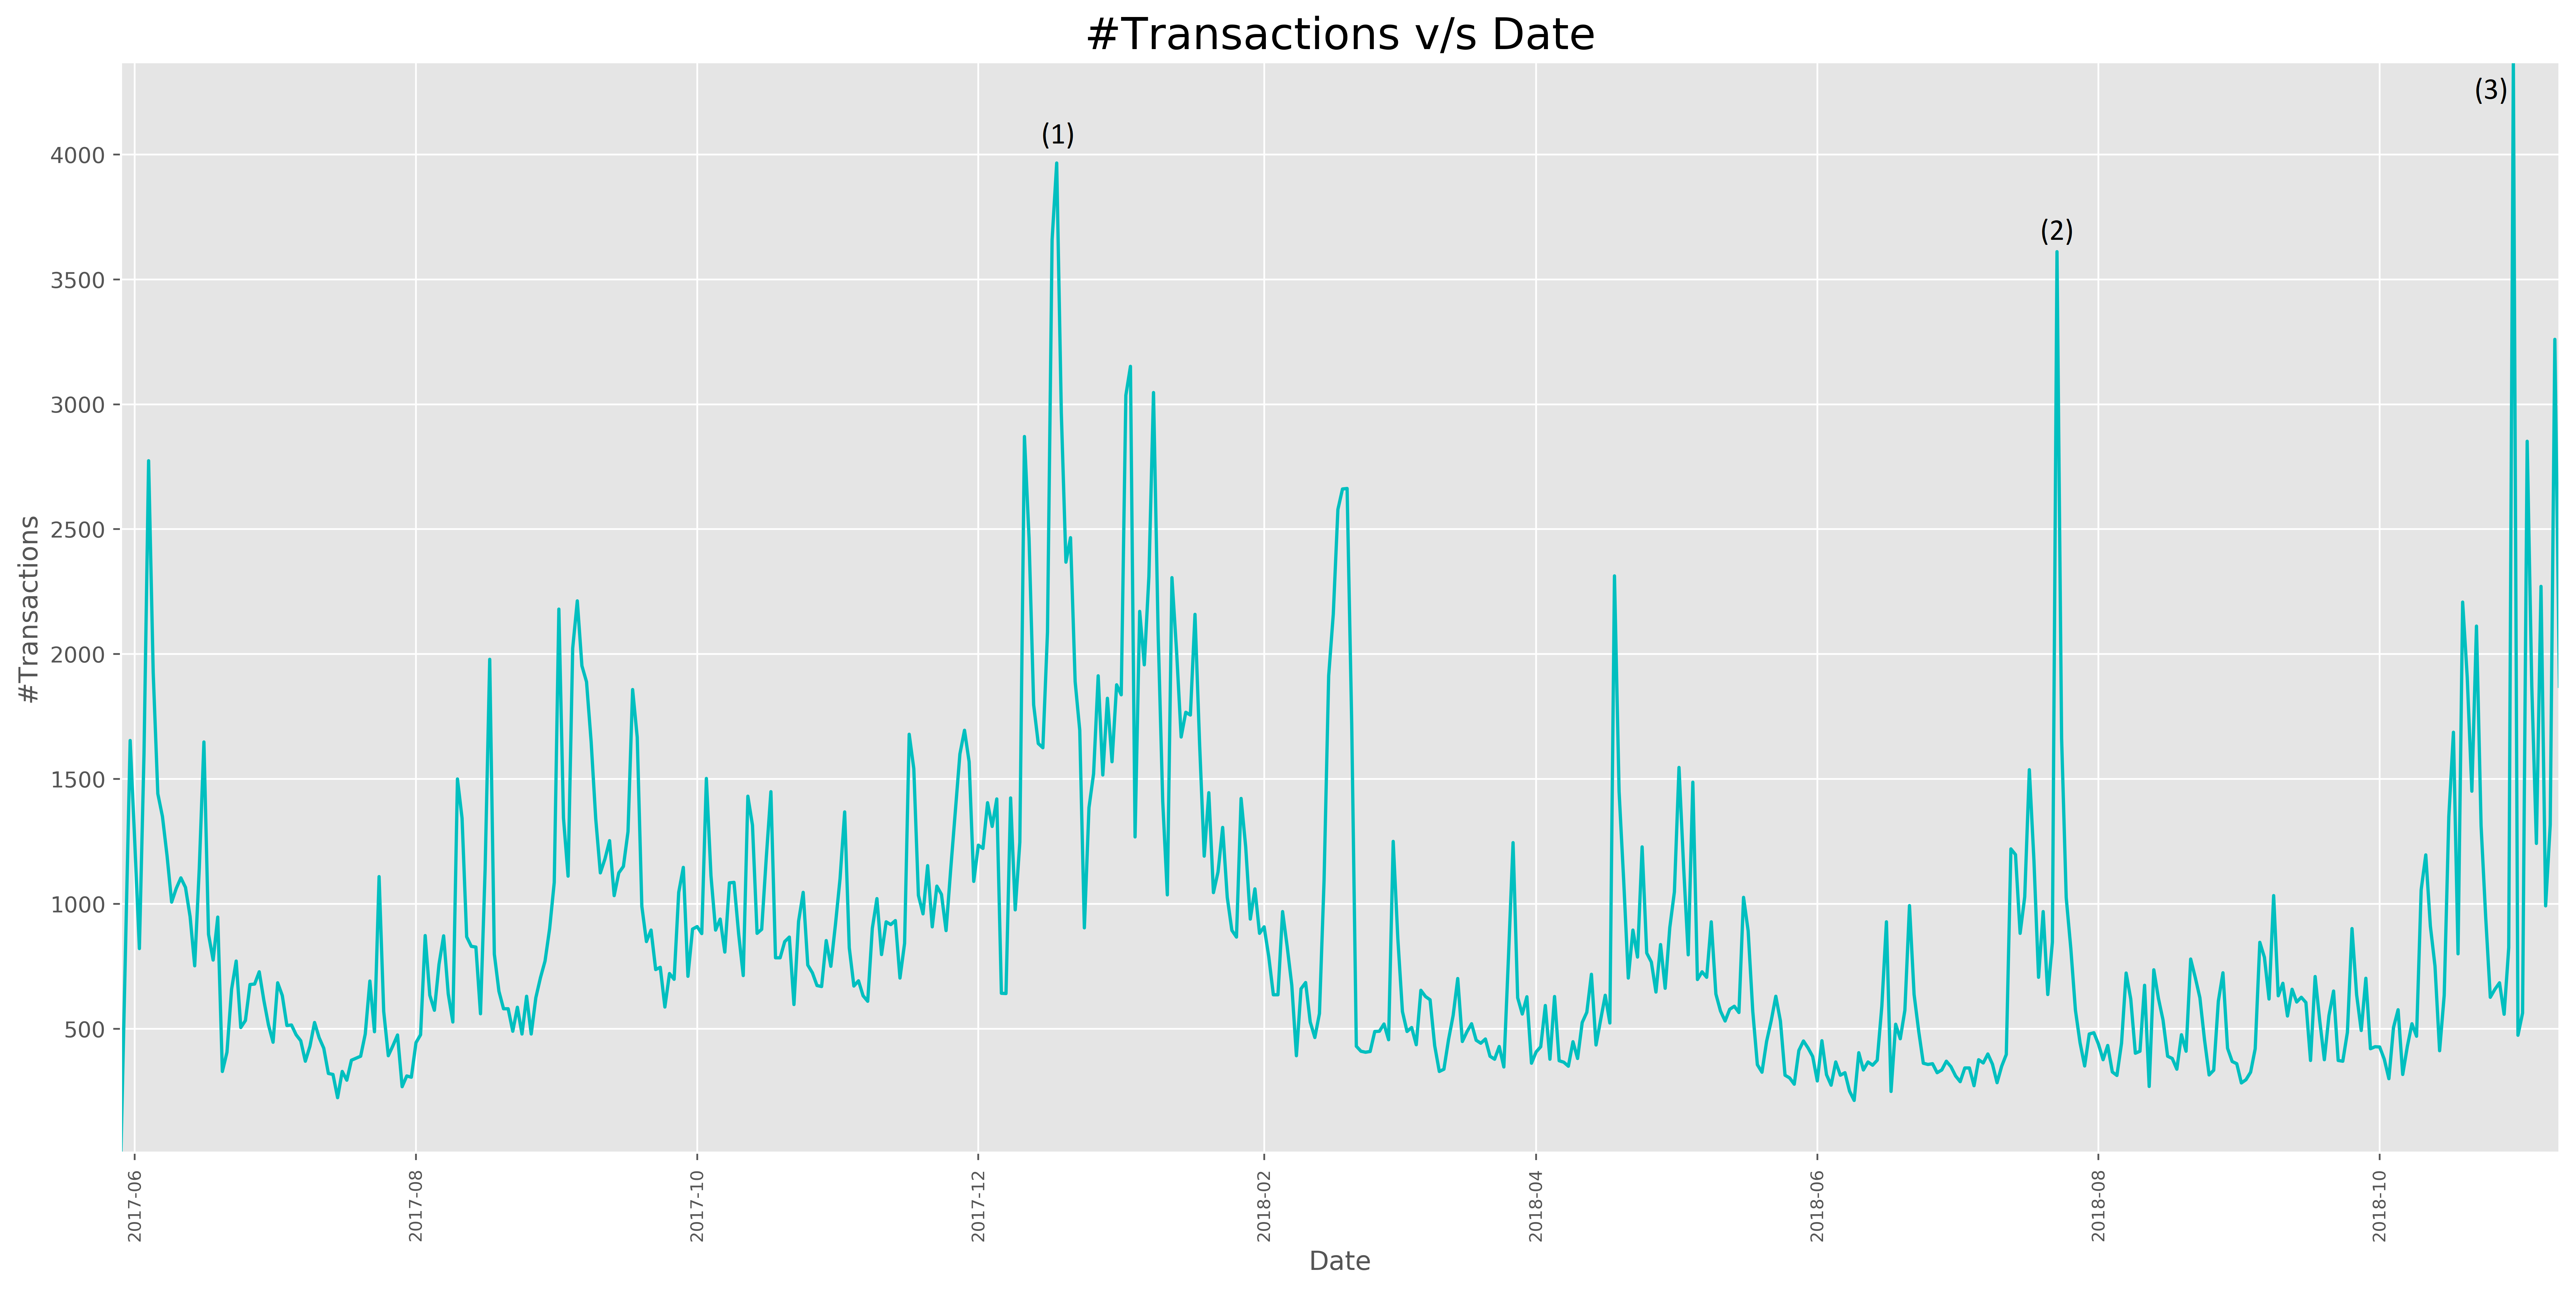
\includegraphics[scale=0.0825]{number-of-Transactions-vs-Date.png}
\caption{Number of transactions per day plotted for over the entire span}
\label{fig:num-txs-vs-date}
\end{figure*}
By analyzing the transfers vs the date, we can observe some interesting
events related to the price of BAT.
Consider the the numbered peaks of Figure \ref{fig:num-txs-vs-date}.
Peak 1 was observed from December 15, 2017 to December 20, 2017.
This was the period while BAT was listed on 4 different exchanges:
Huobi Pro, zb.com, Bifinex, Coinhood.
The investors might have predicted the price of BAT to
rise, and so perhaps they all started sending many transfers in/out of
the exchanges, and this increased the number of transactions.
Peak 2 was observed on July 23, 2018 and we could not find any events
to associate with this drastic rise in the number of transactions.
Peak 3 was observed from October 31, 2018 to November 3, 2018.
BAT was listed on Coinbase Pro somewhere around this time,
and so it is probable that
1) news of this listing probably circulated before the BAT was actually listed,
and 2) many investors predicted a change in price, and thus
started sending many transfer in/out of the exchanges.
Finally, we observed from the data that the average value of
BAT transfers started off very high after the ICO (as expected),
and then generally decreased over time.

% \begin{figure}
% 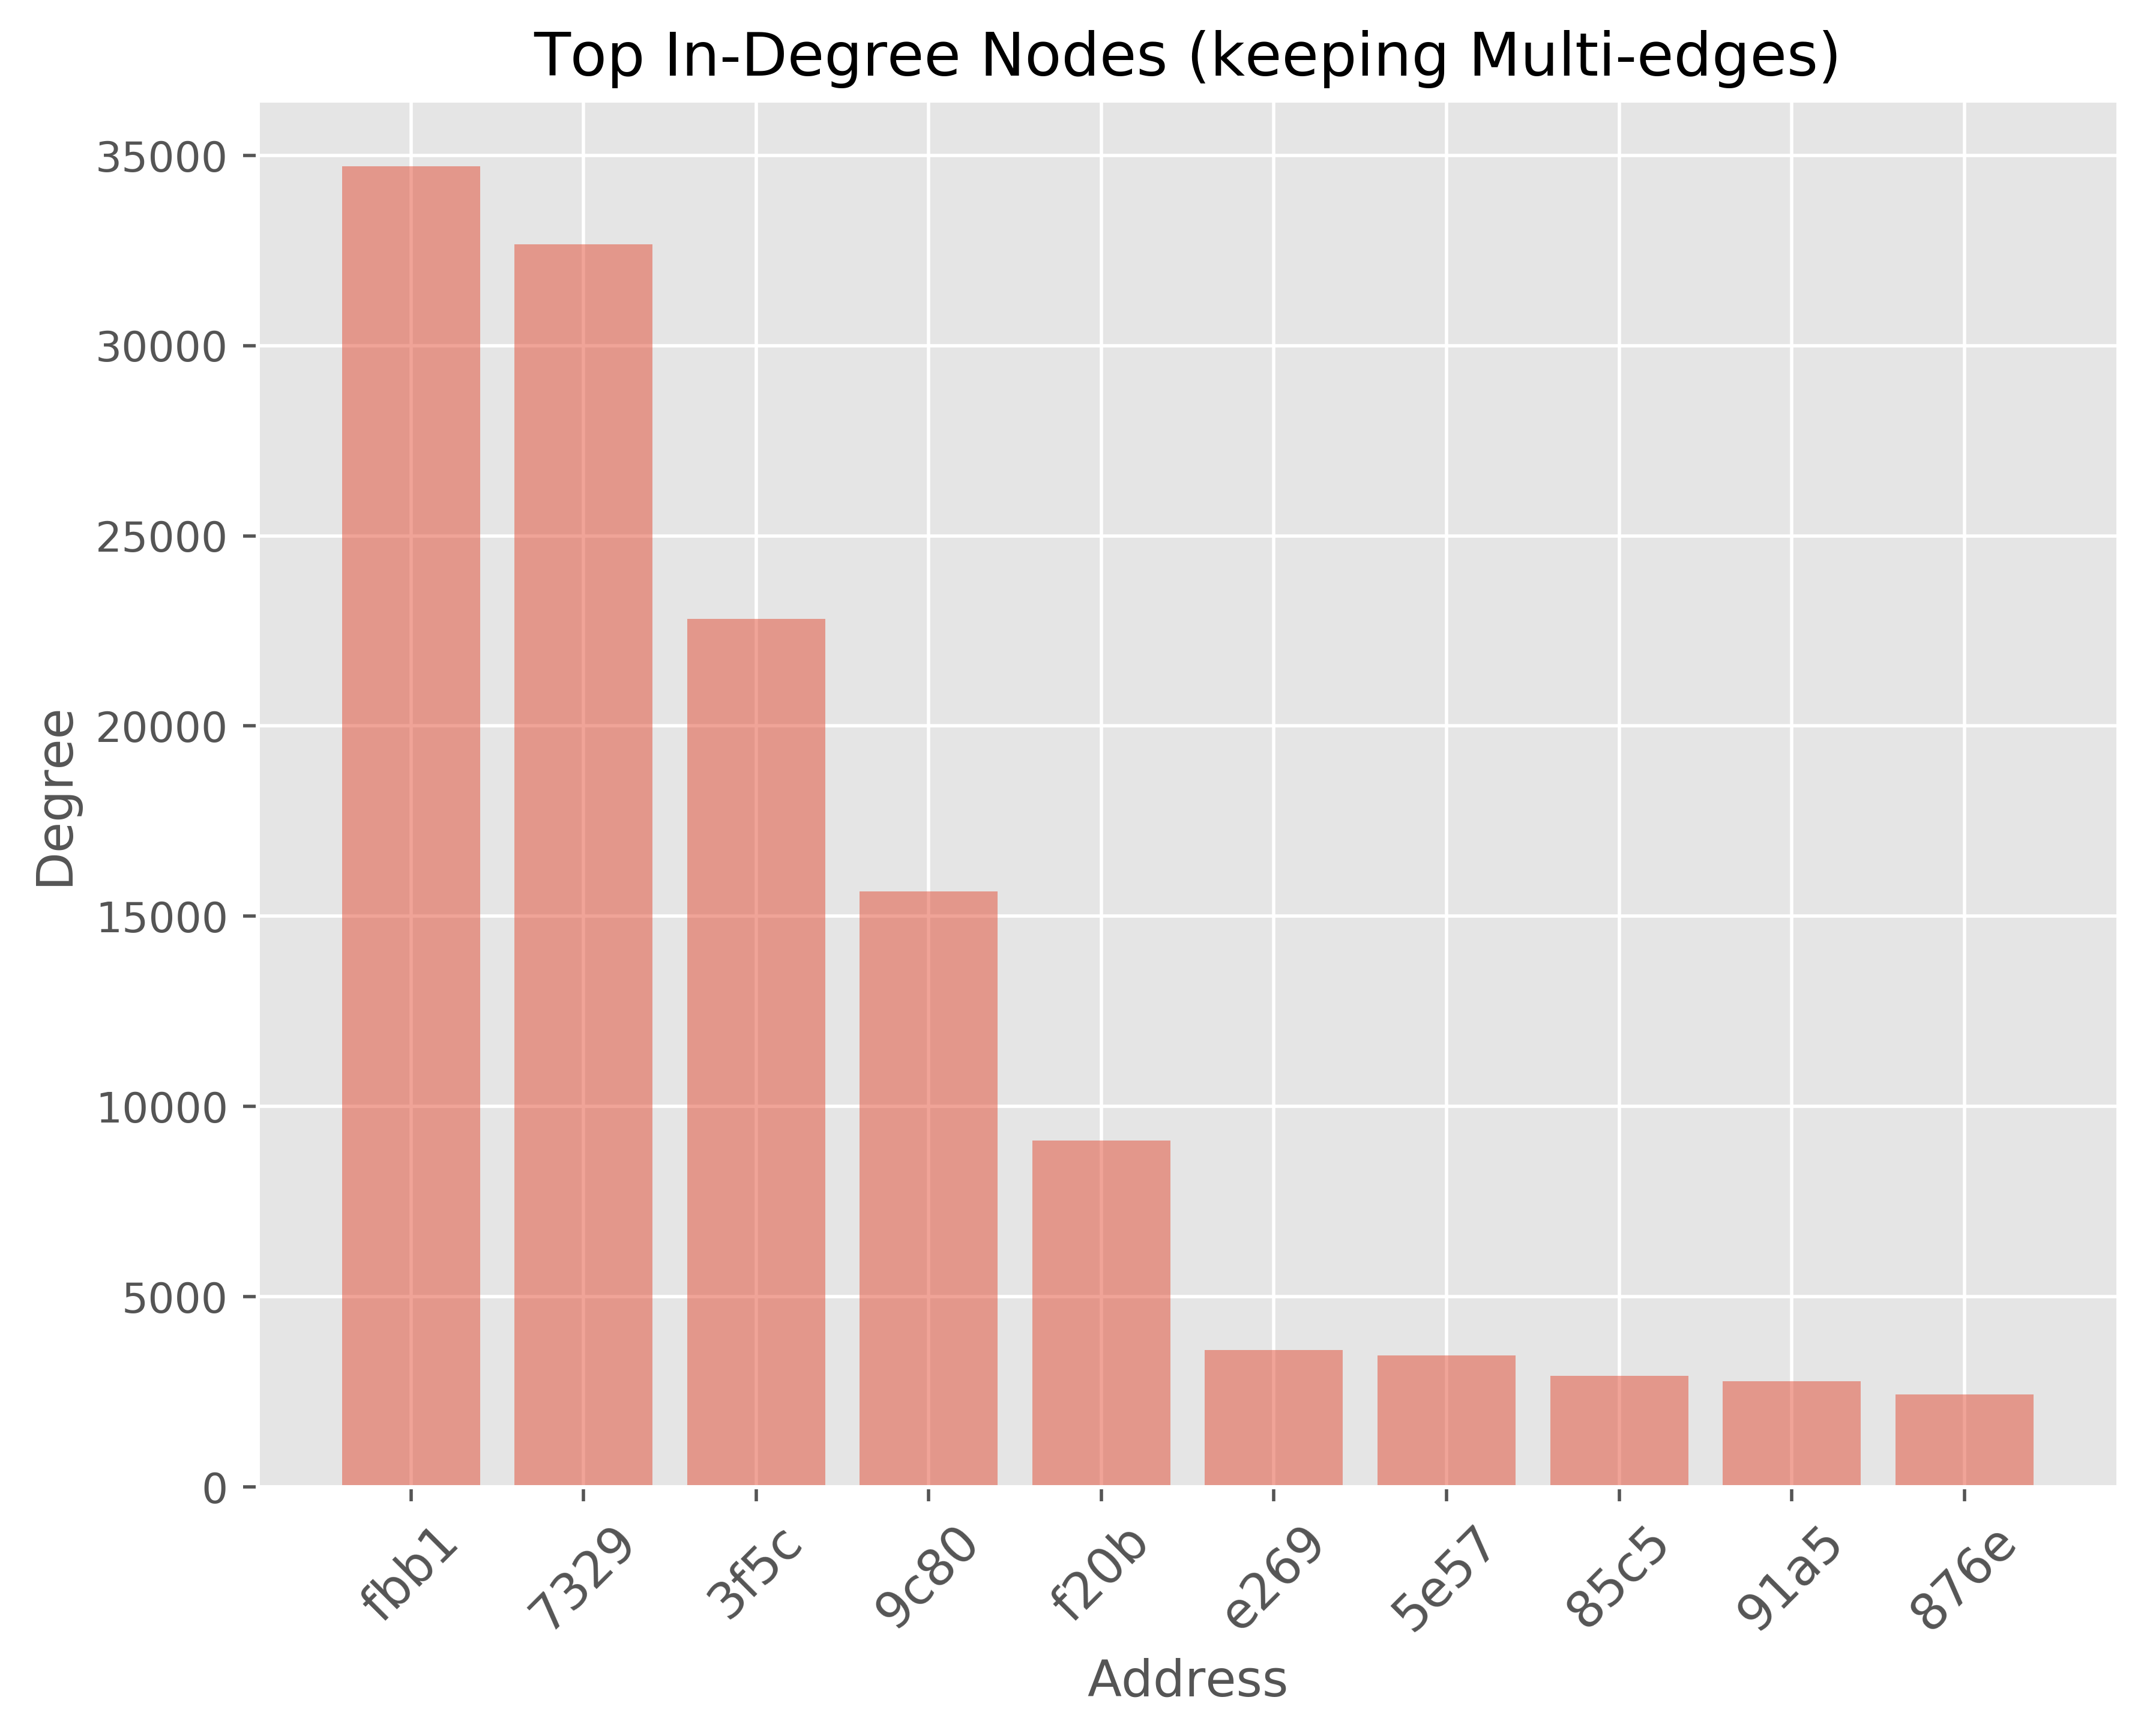
\includegraphics[scale=0.5]{Top_In-Degree_Nodes_(keeping_Multi-edges).png}
% \end{figure}

% \begin{figure}
% 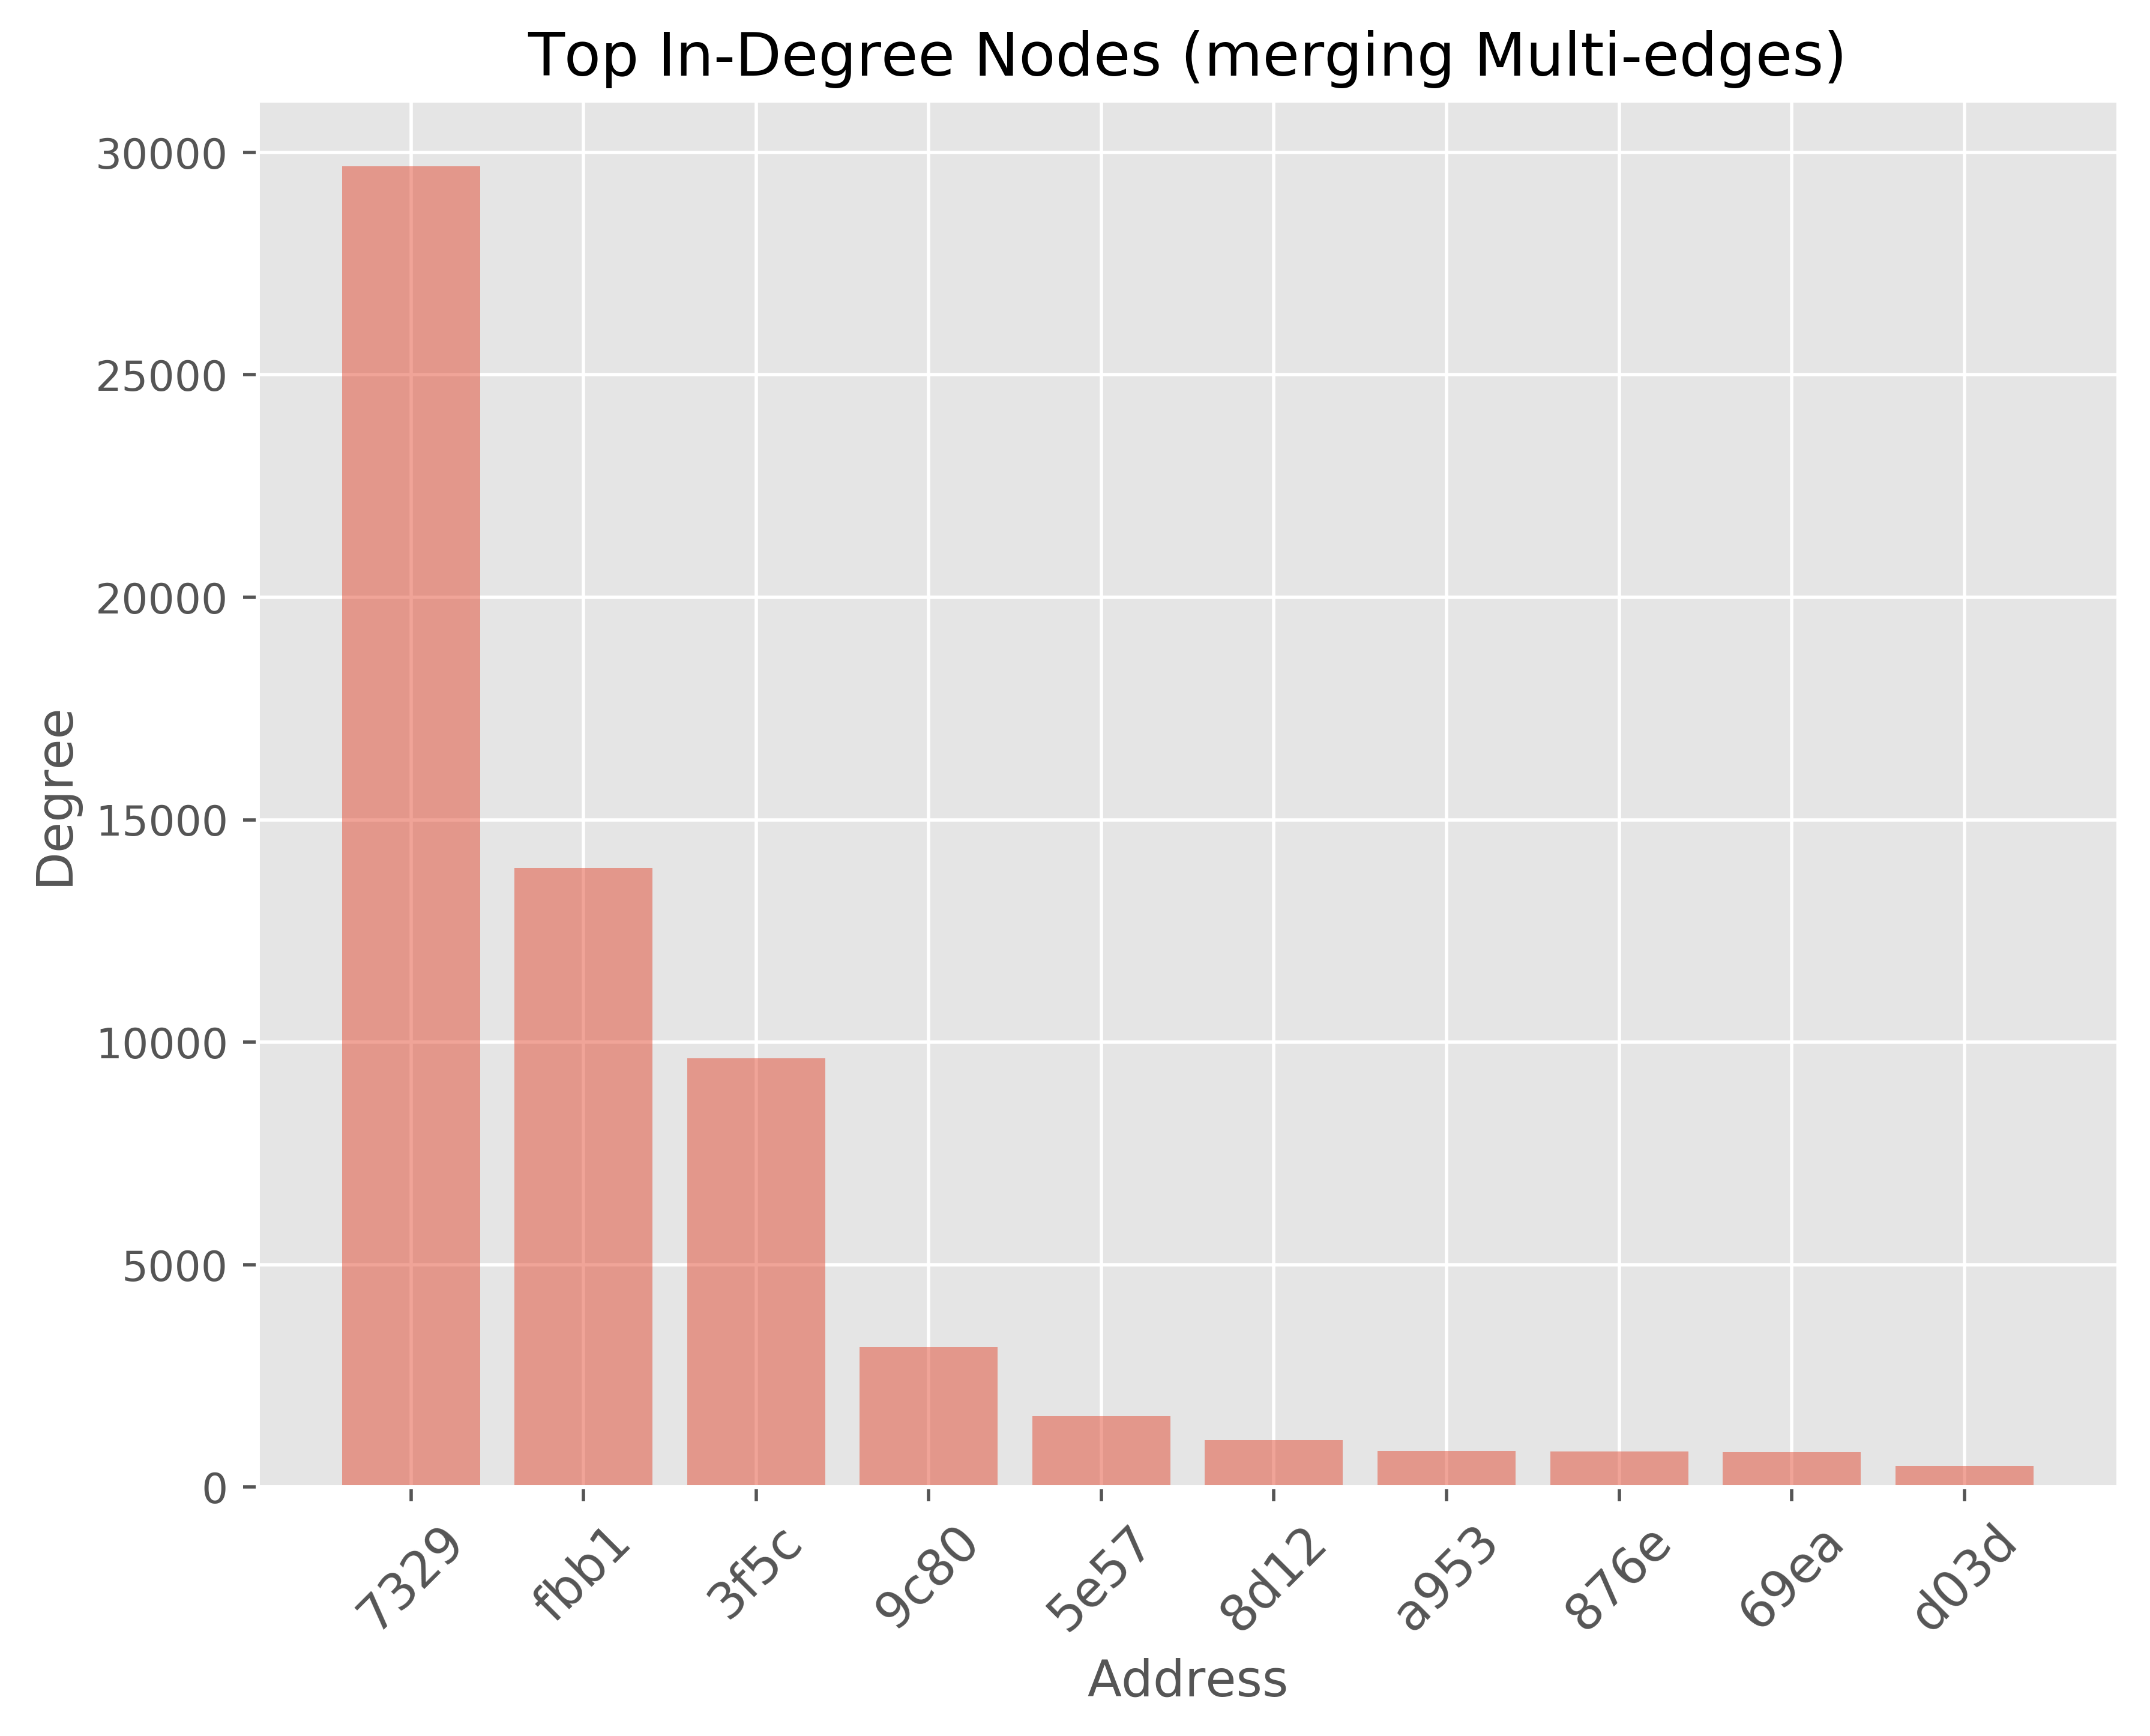
\includegraphics[scale=0.5]{Top_In-Degree_Nodes_(merging_Multi-edges).png}
% \end{figure}

% \begin{figure}
% 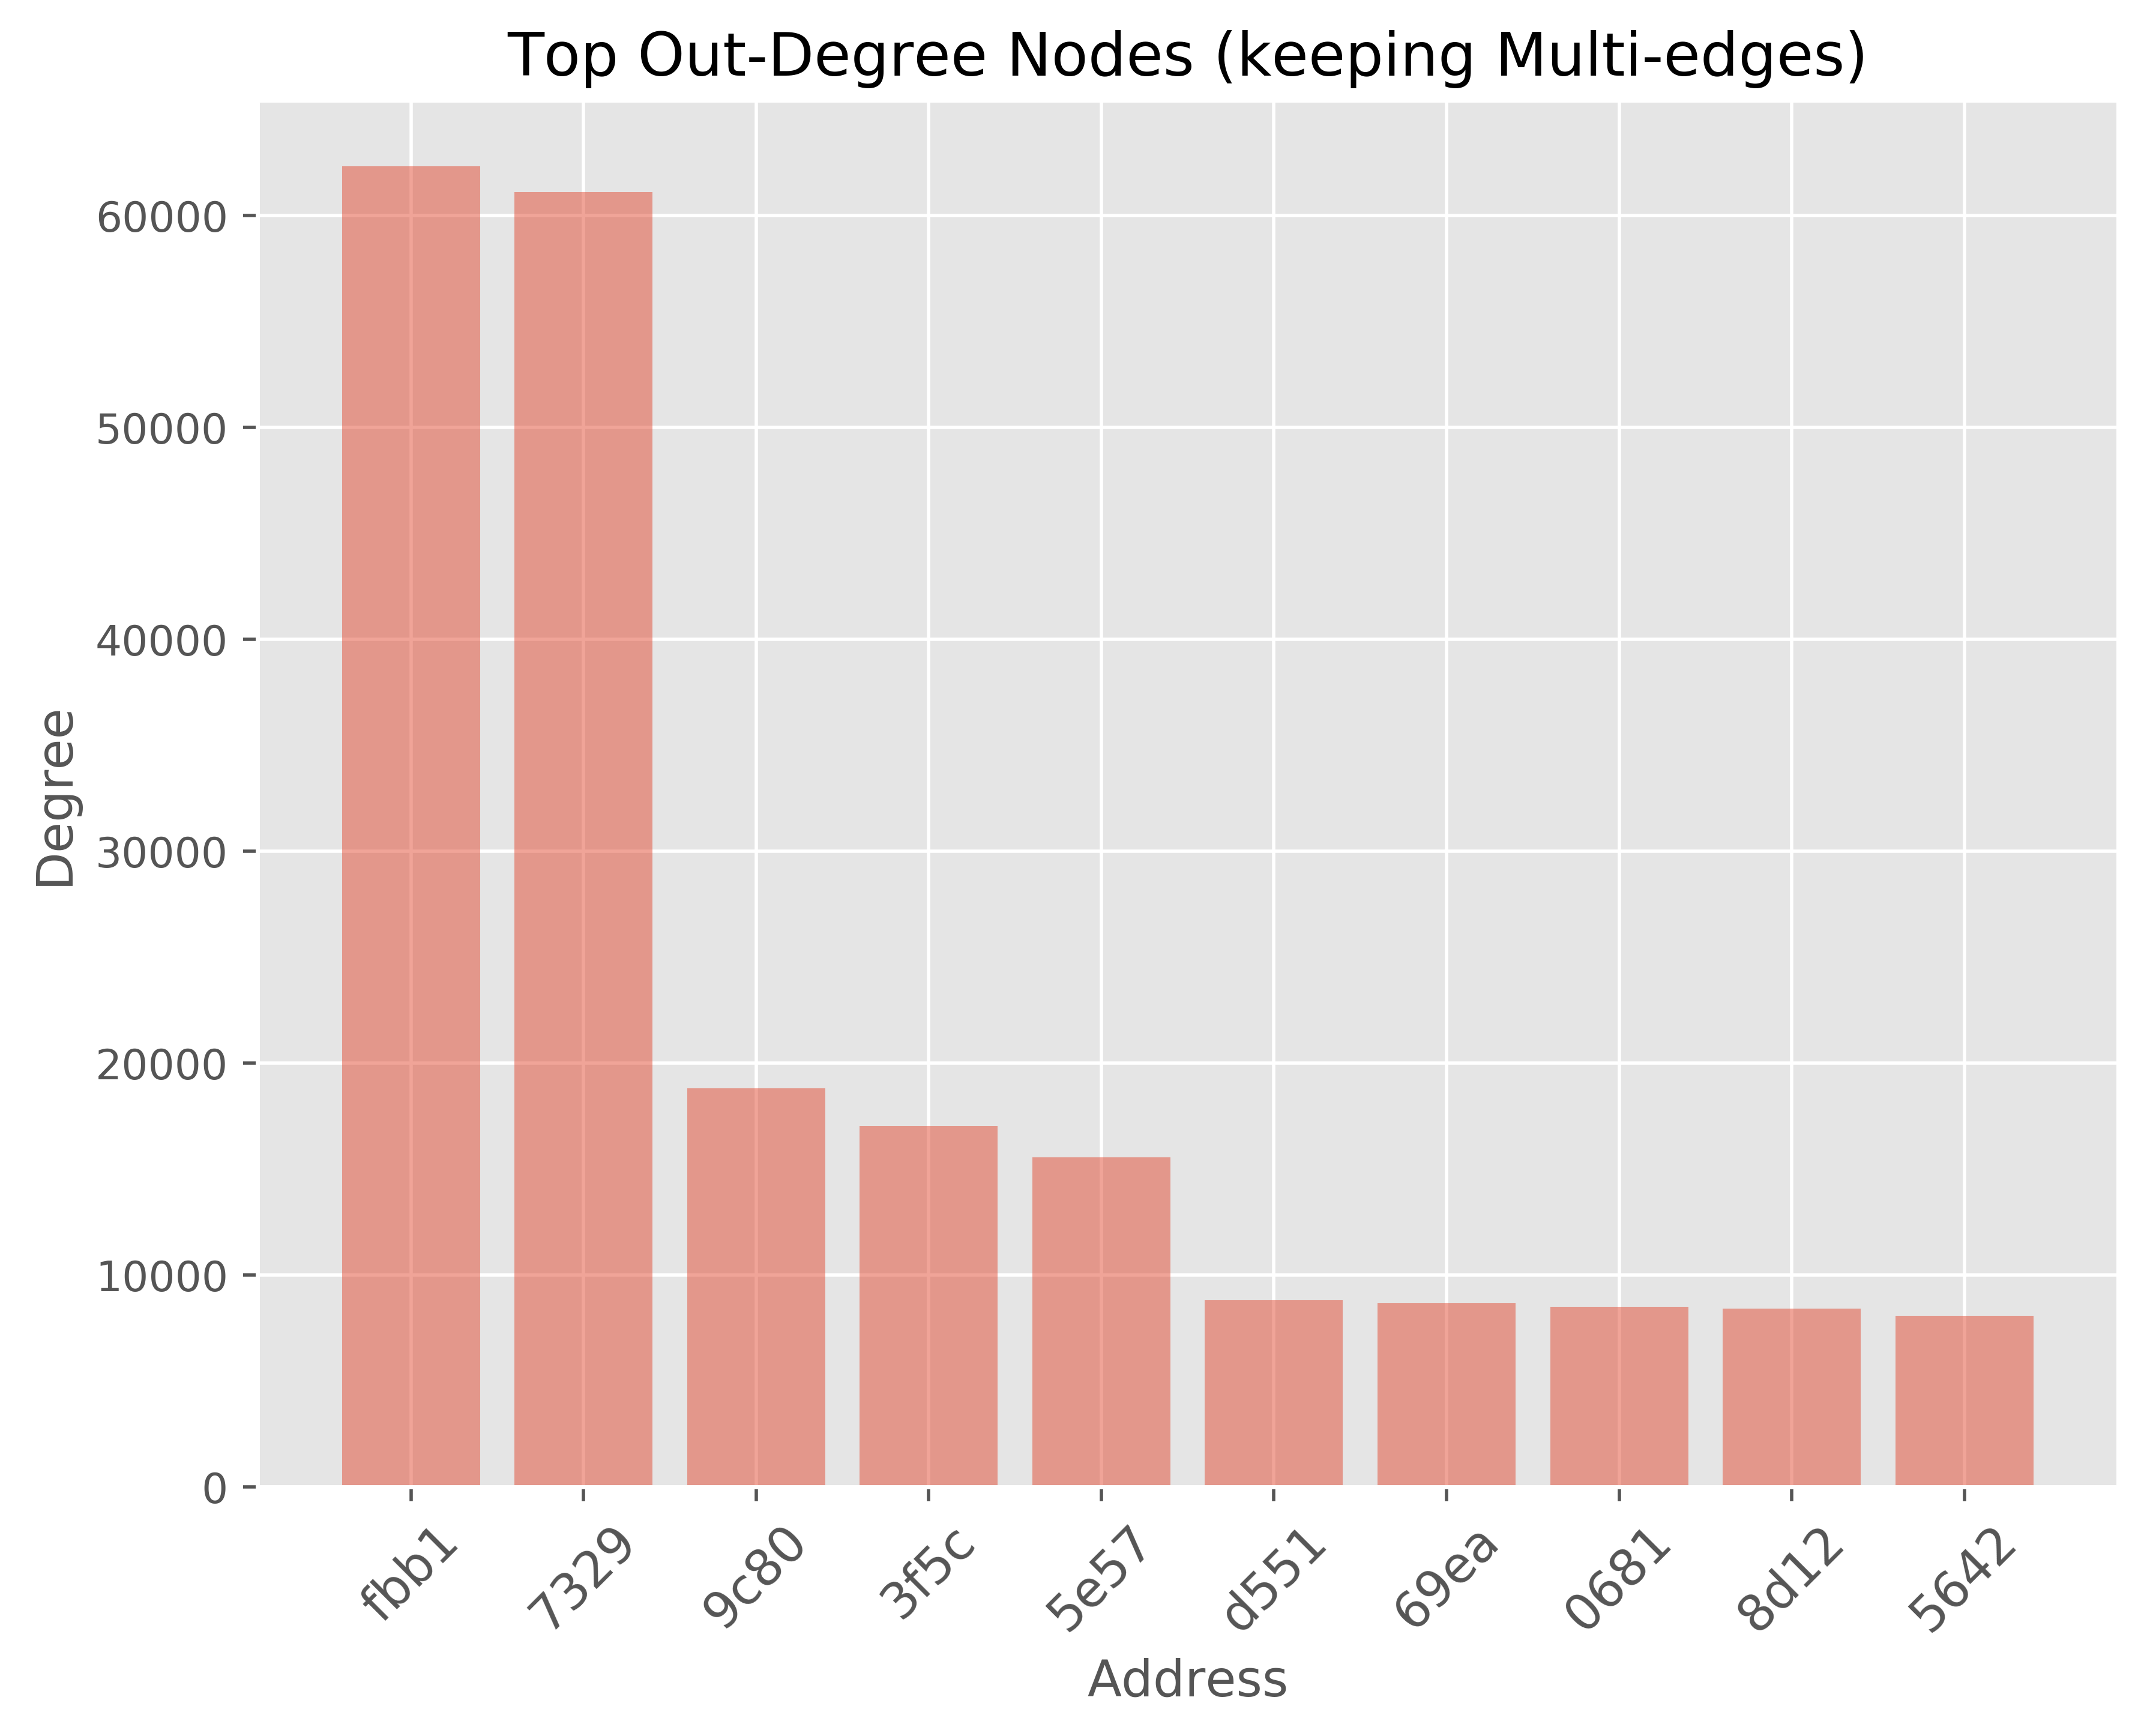
\includegraphics[scale=0.5]{Top_Out-Degree_Nodes_(keeping_Multi-edges).png}
% \end{figure}

% \begin{figure}
% 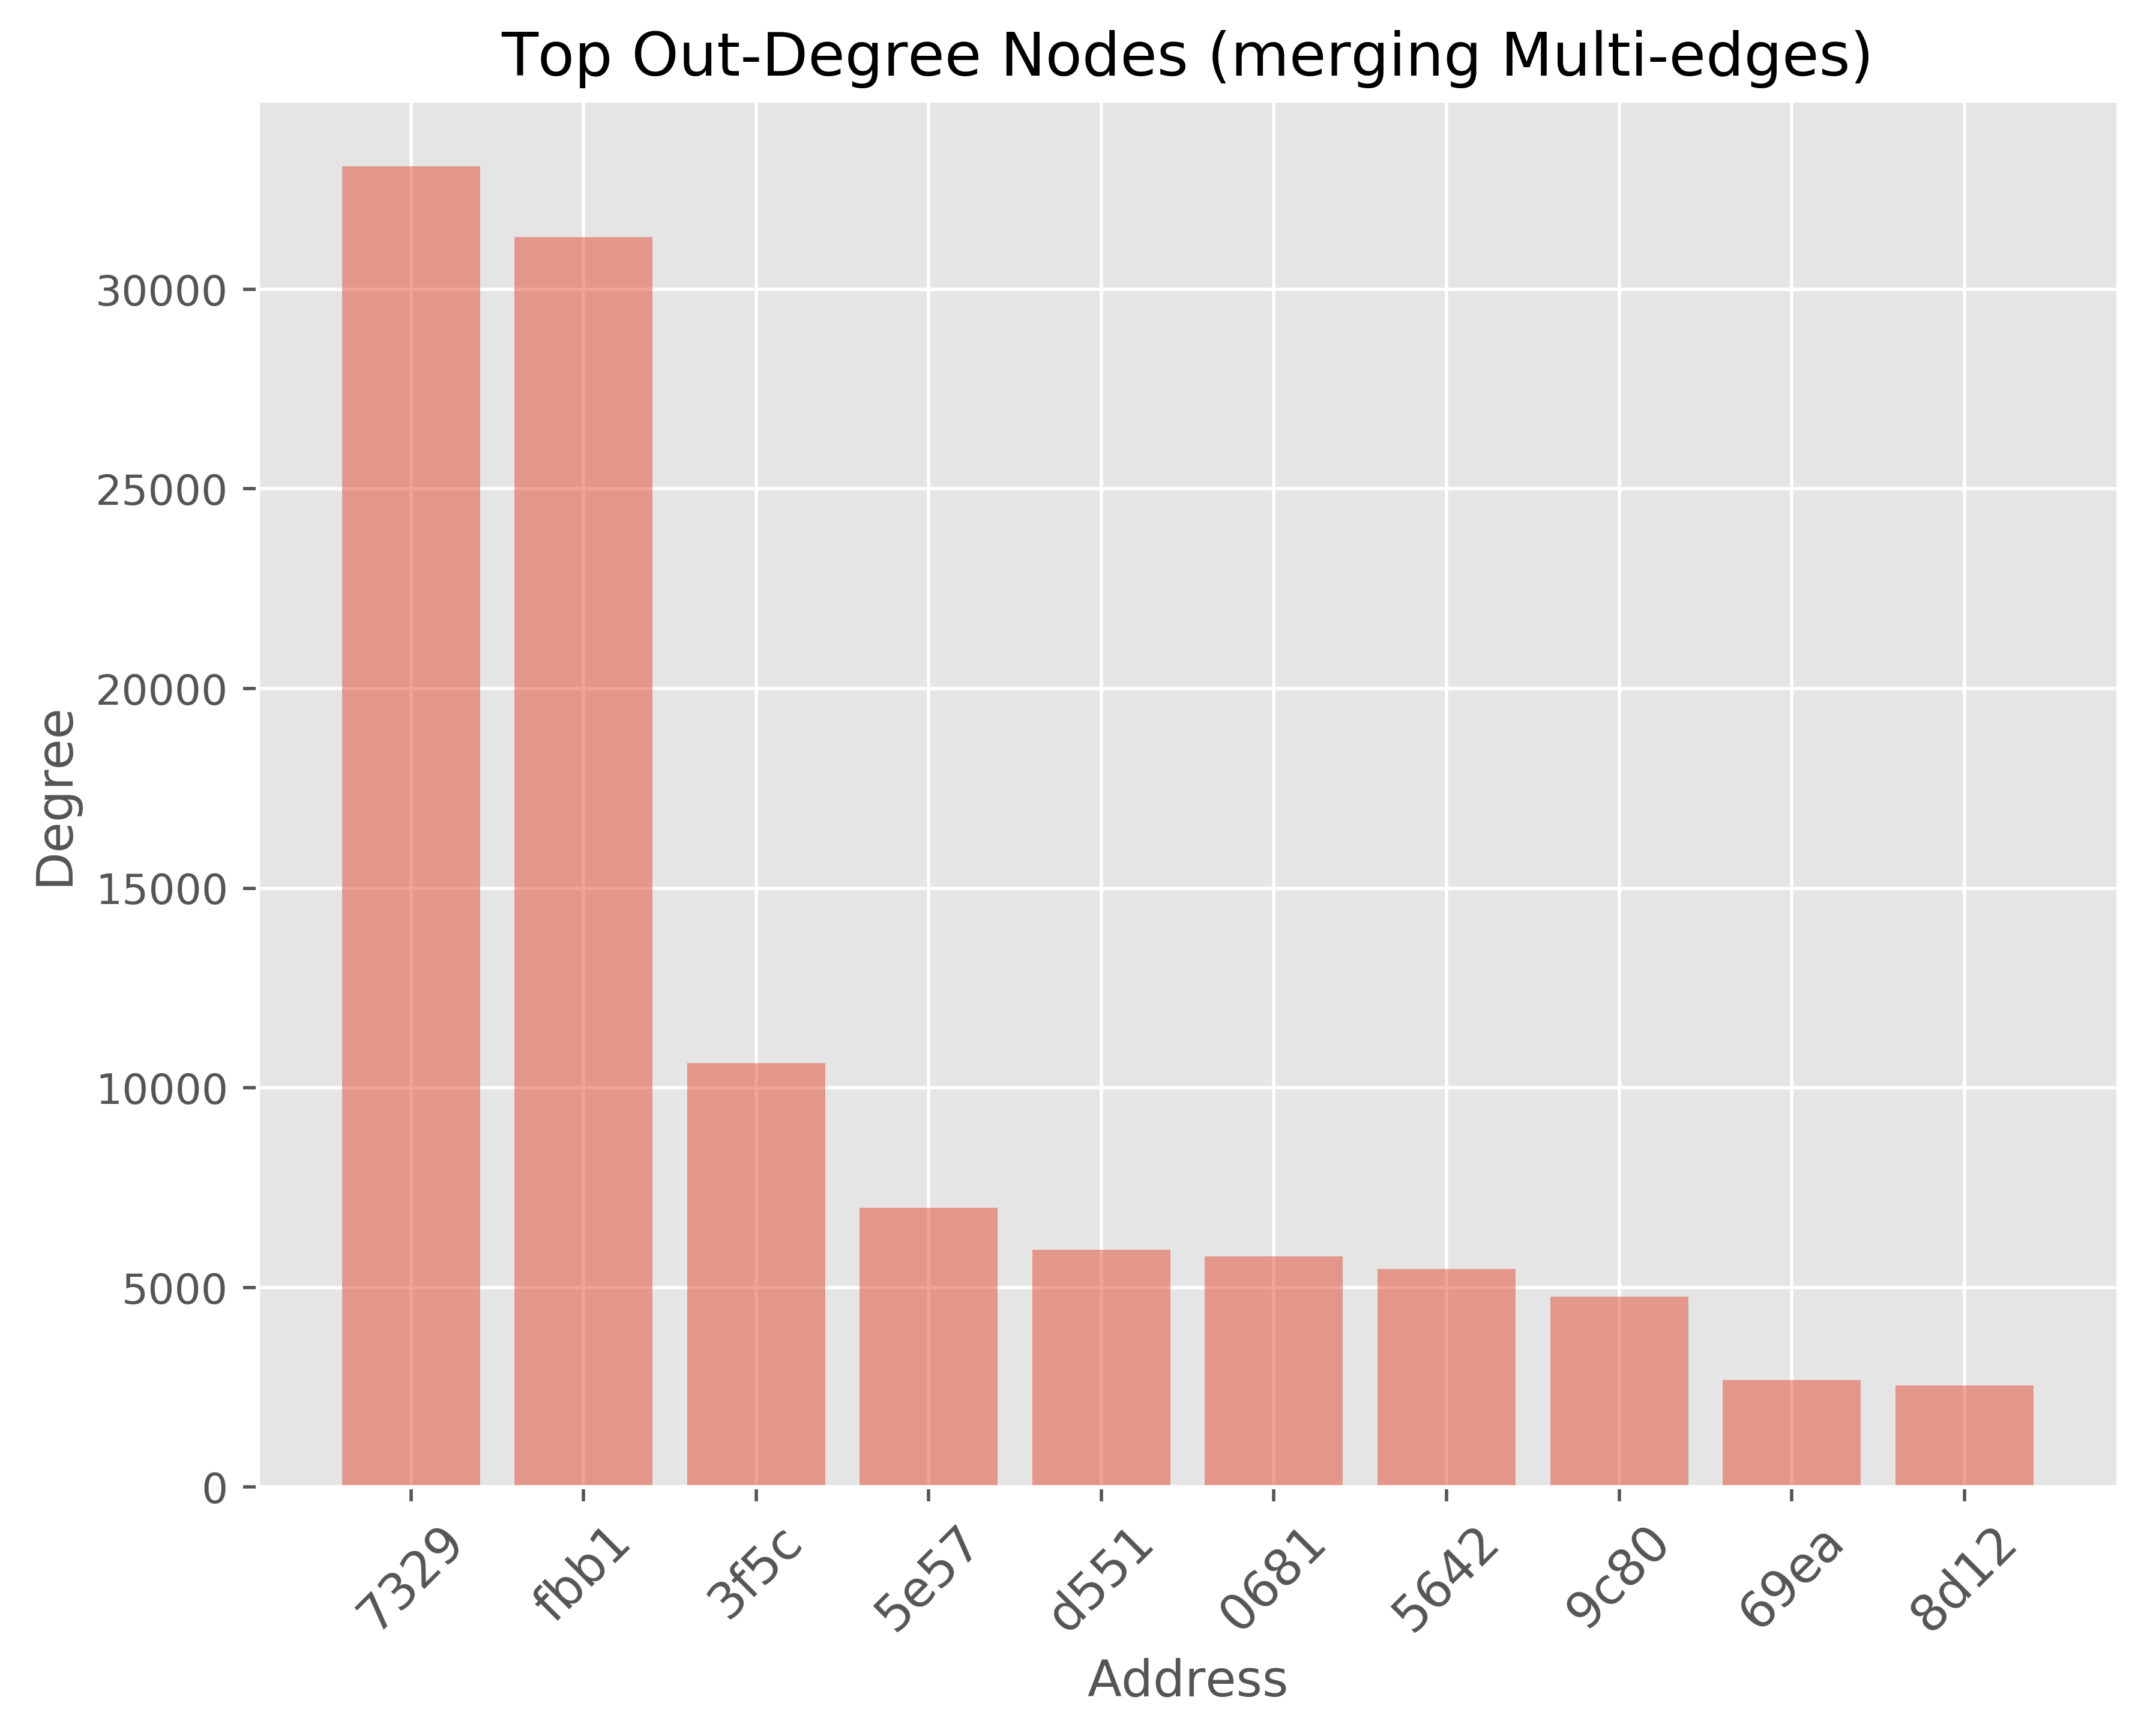
\includegraphics[scale=0.5]{Top_Out-Degree_Nodes_(merging_Multi-edges).png}
% \end{figure}

\begin{figure*}
\begin{tabular}{cc}%
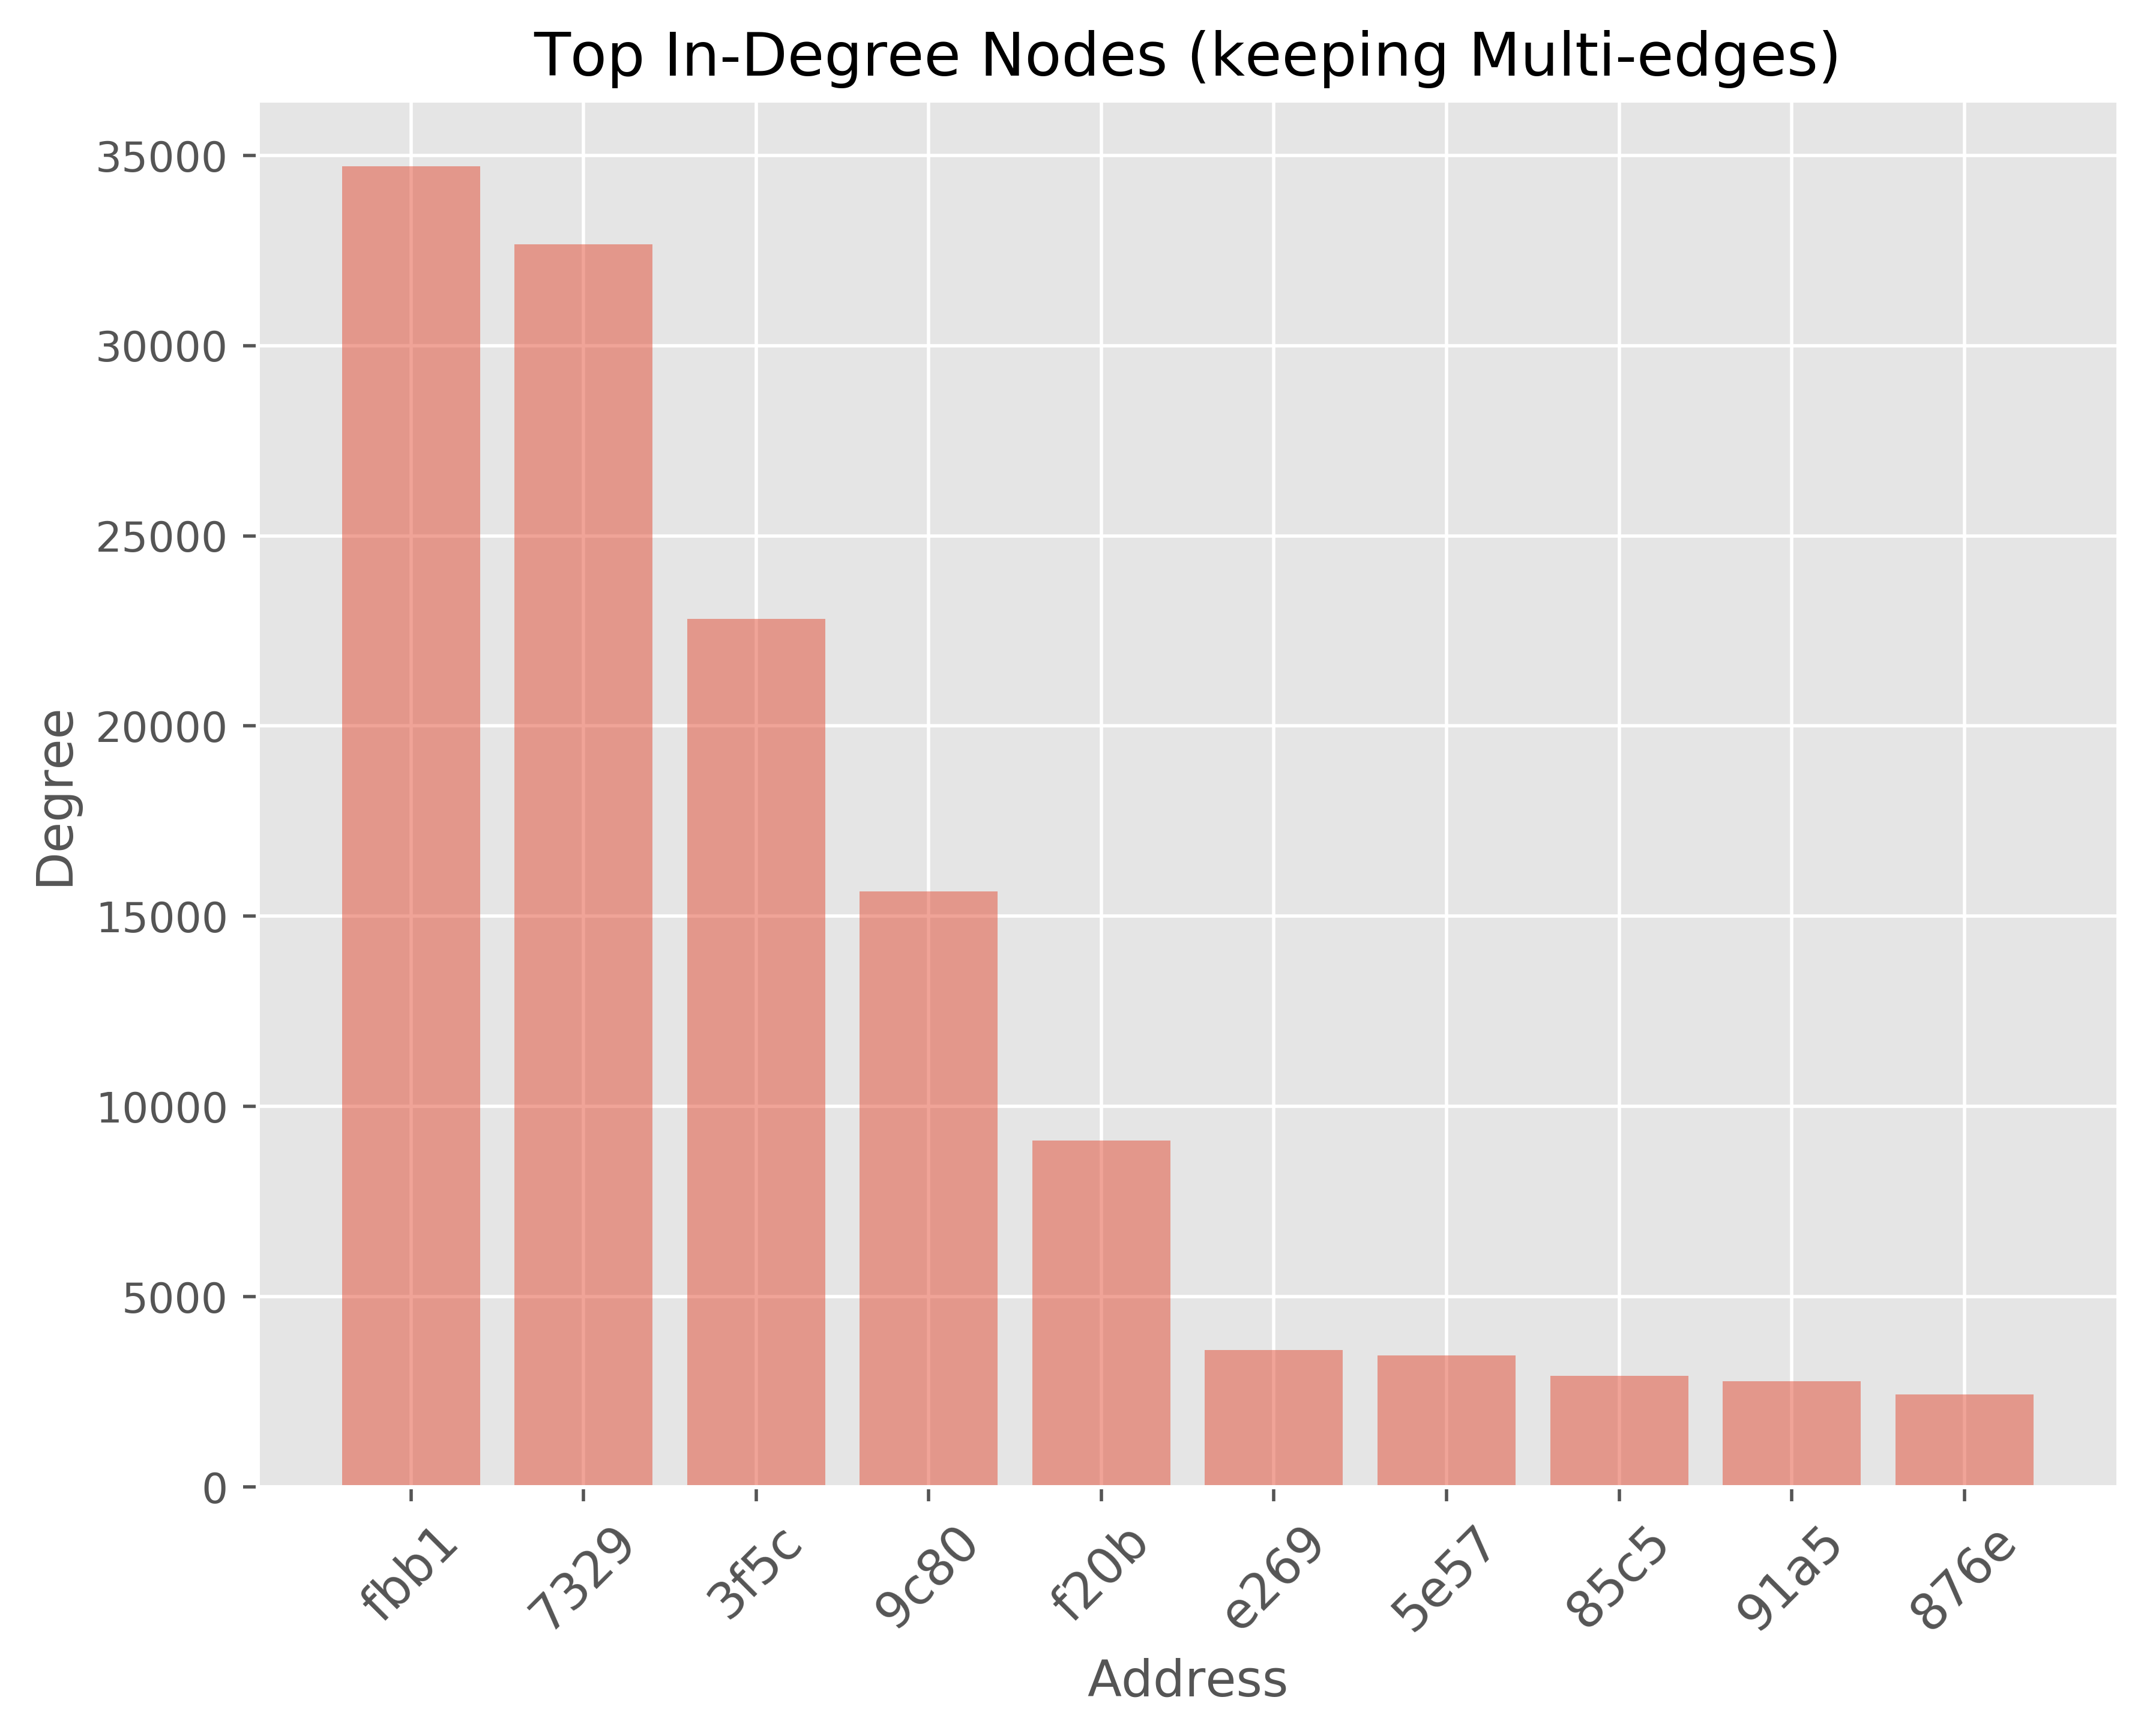
\includegraphics[scale=0.4]{Top_In-Degree_Nodes_(keeping_Multi-edges).png}&
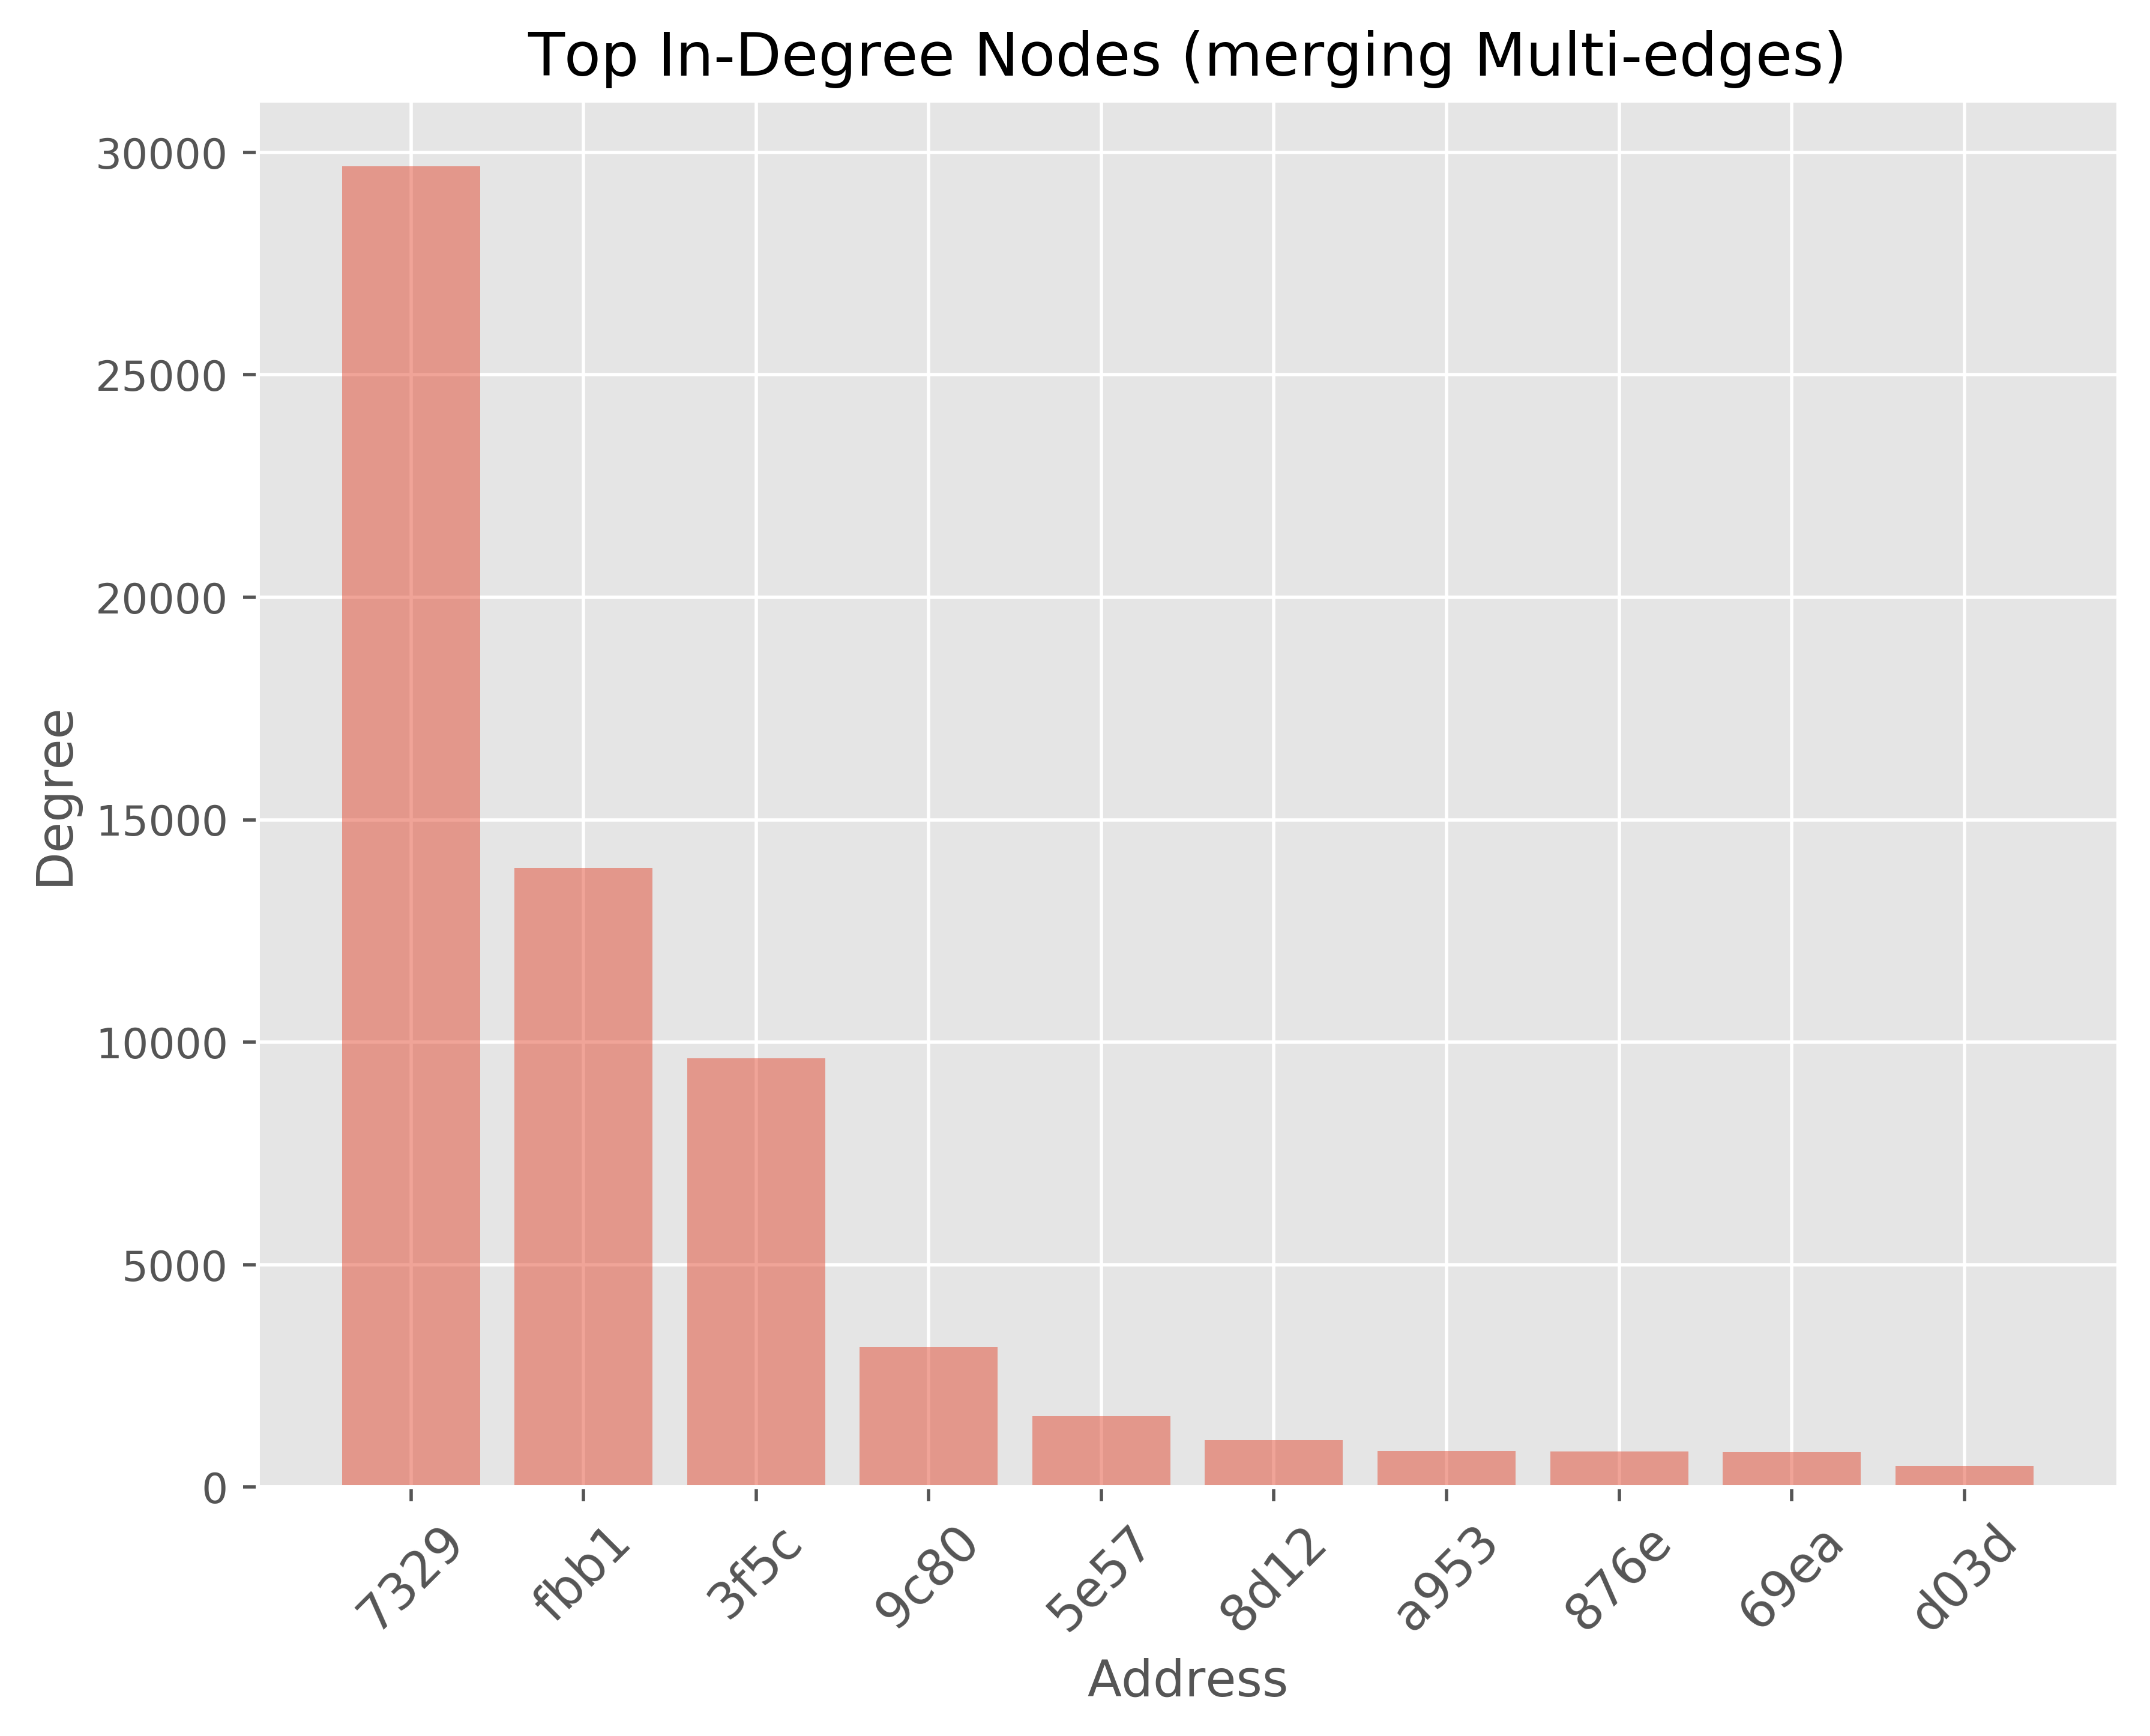
\includegraphics[scale=0.4]{Top_In-Degree_Nodes_(merging_Multi-edges).png}\\
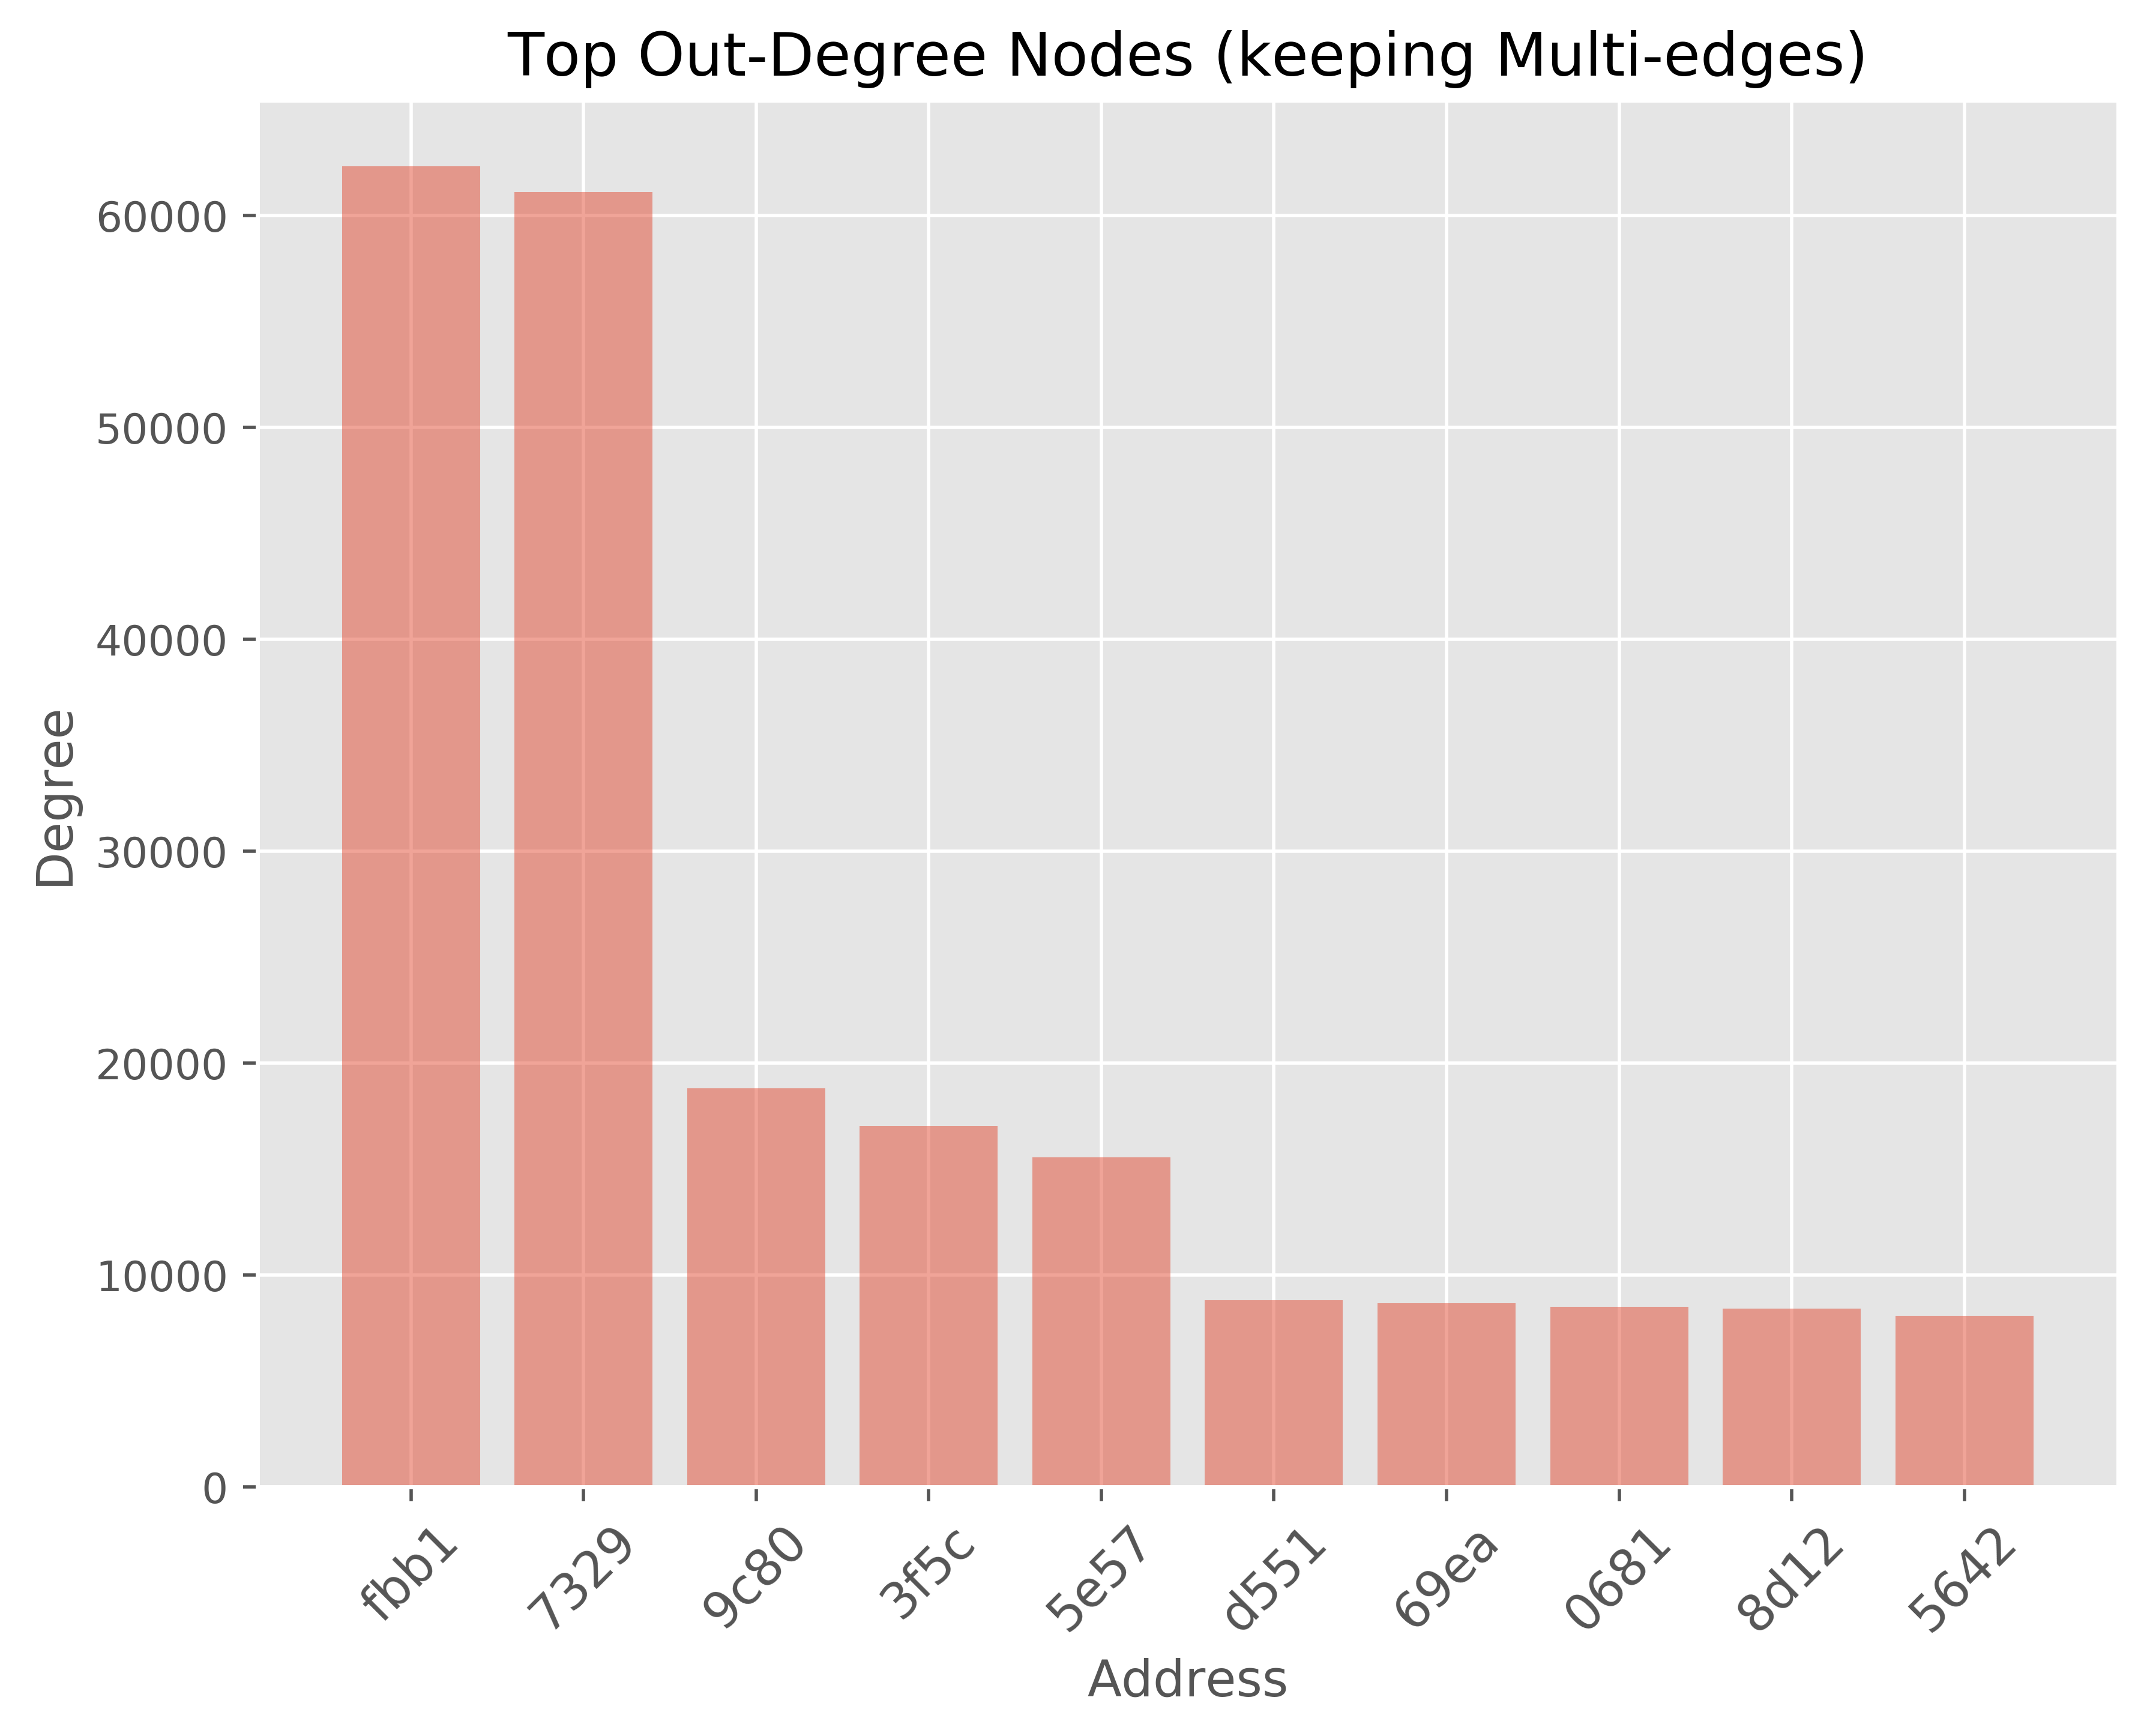
\includegraphics[scale=0.4]{Top_Out-Degree_Nodes_(keeping_Multi-edges).png}&
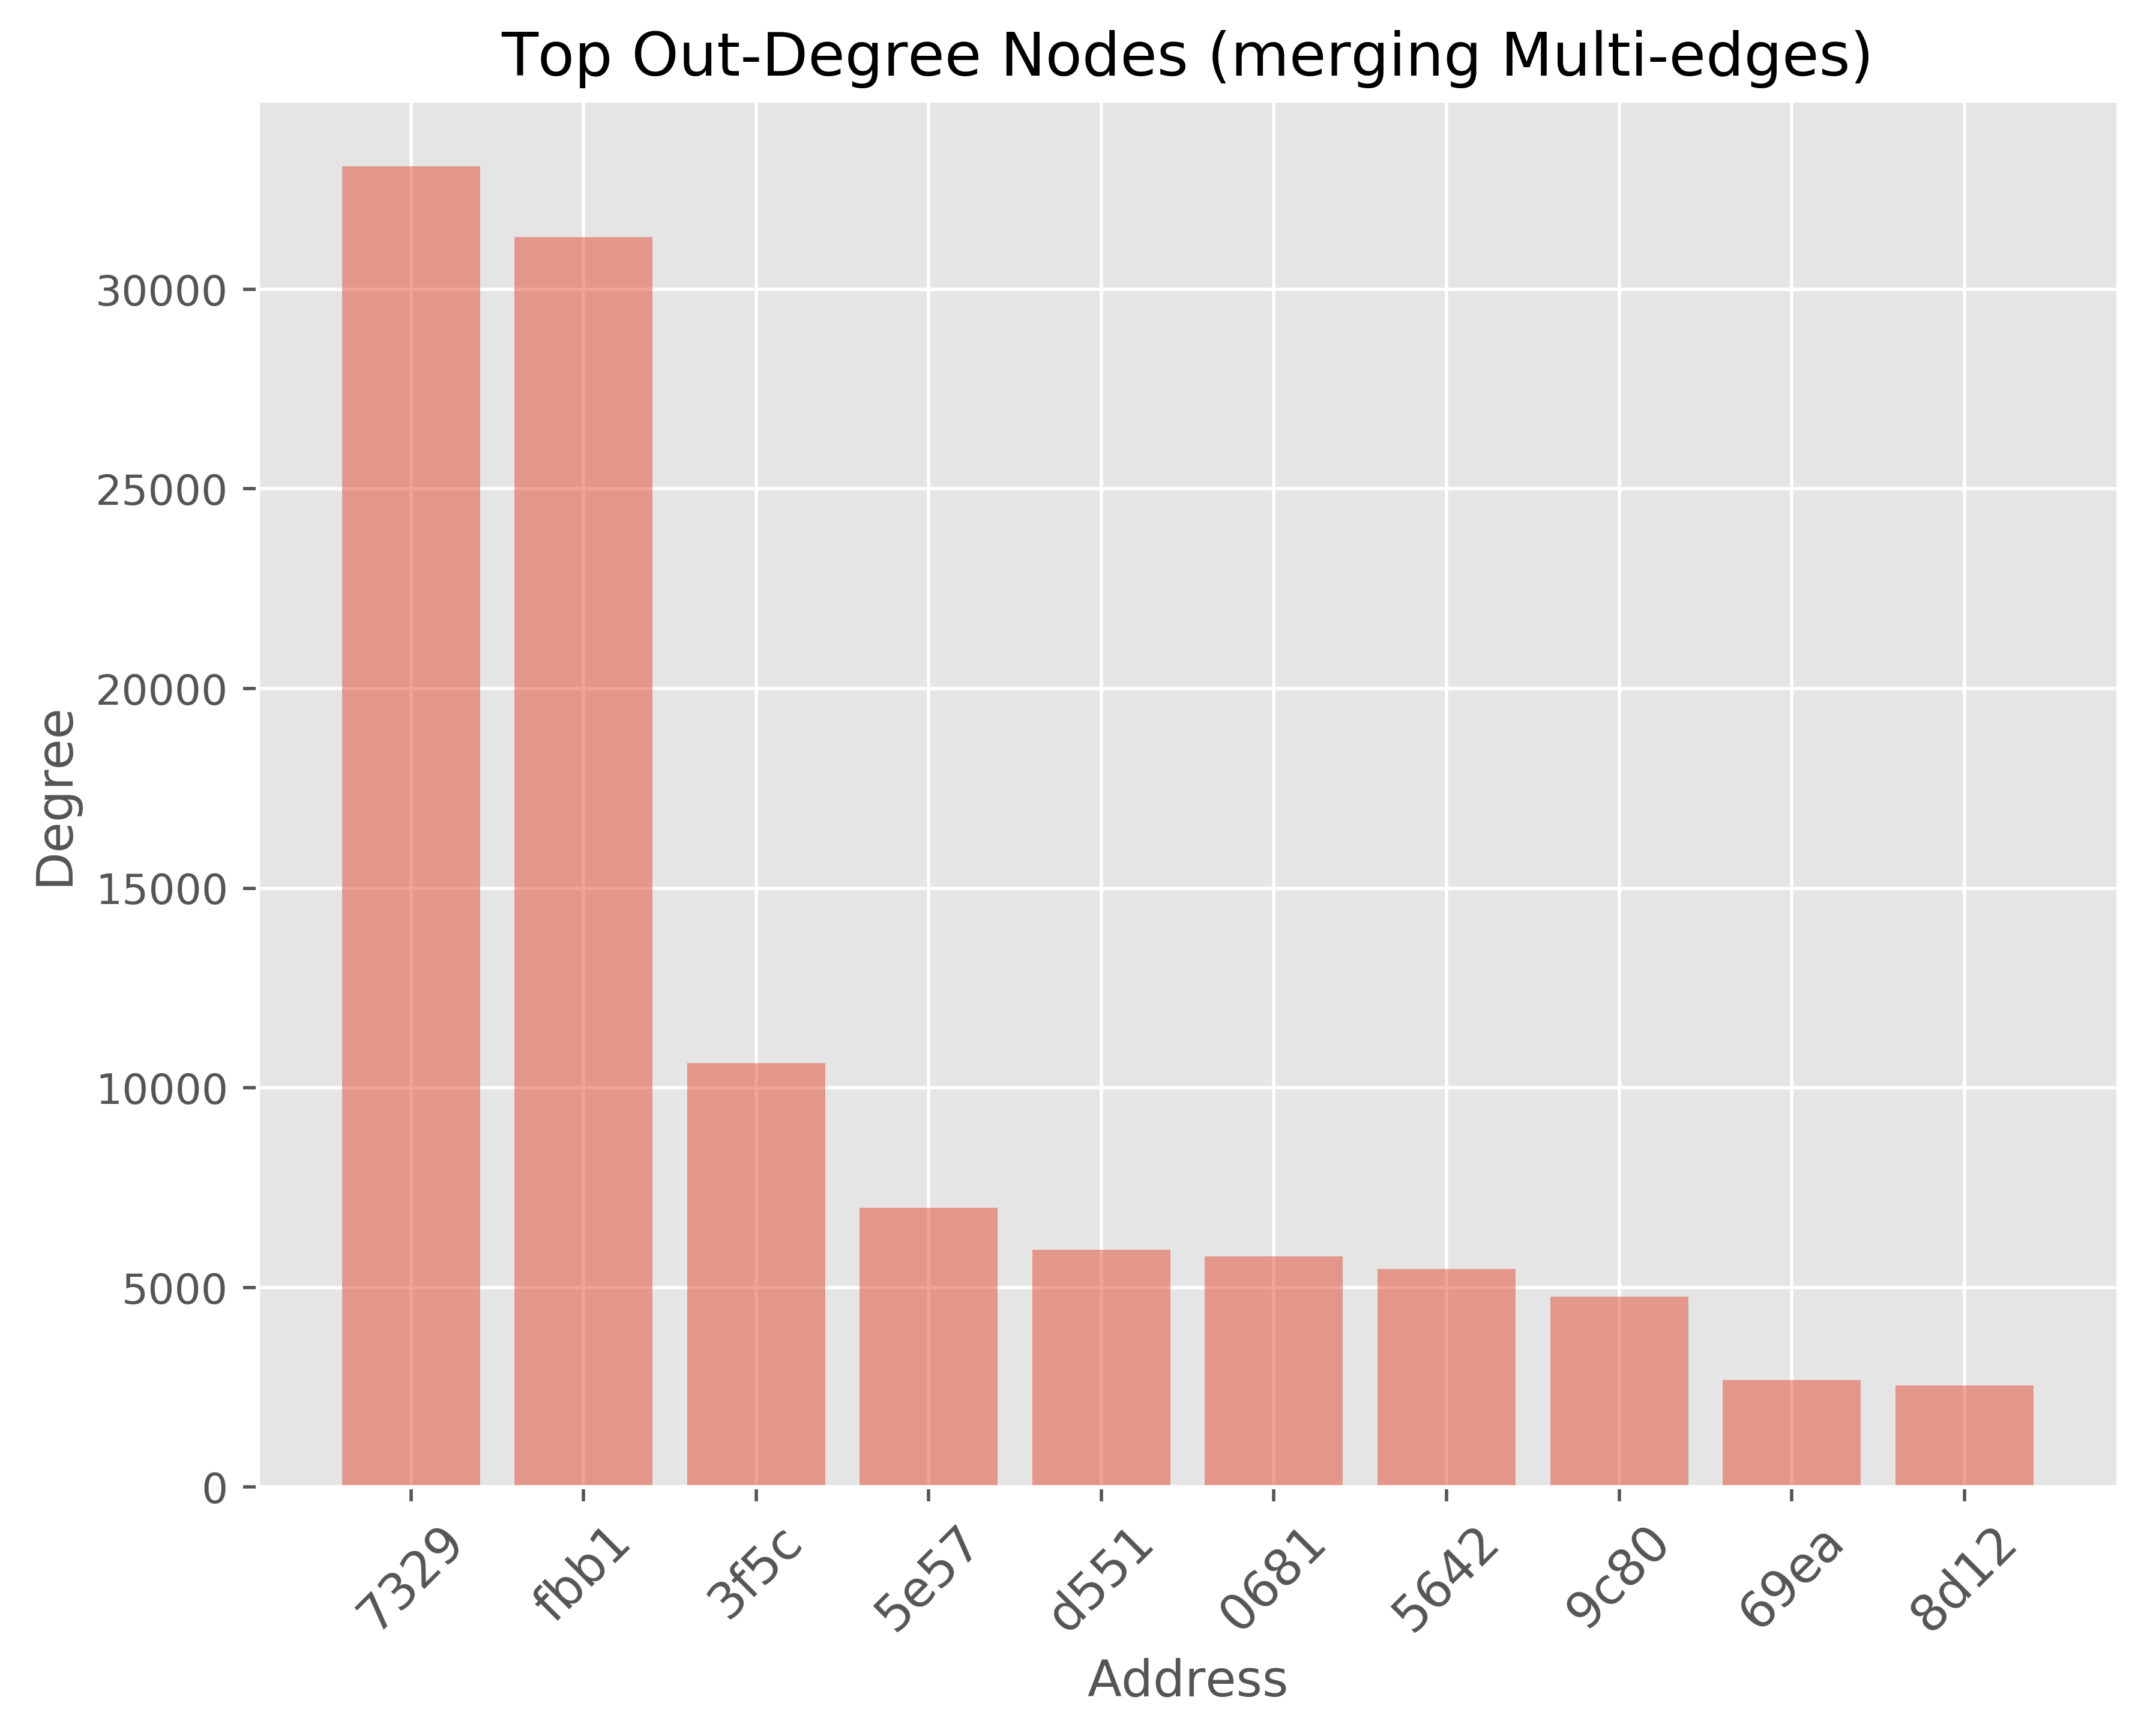
\includegraphics[scale=0.4]{Top_Out-Degree_Nodes_(merging_Multi-edges).png}\\
\end{tabular}
\caption{Top addresses with in-degrees and out-degrees keeping the multi-edges and merging the multi-edges over the entire span.}
\label{fig:inout-degrees}
\end{figure*}
All the 4 plots in Figure \ref{fig:inout-degrees} share addresses from a set of 15 addresses with the top addresses remaining the same for all of the graphs.
These addresses are probably owned by different exchanges (only a few could be labeled), which explains such high in and out degrees.
It can be noted from the graphs that address ``0xfbb1b73c4f...''
has the highest in-degree without merging multi-edges (around 35,000).
With merging multi-edges the in-degree falls to around 14,000.
This shows that there are \emph{some} addresses that
execute multiple transactions to/from this address.
The address ``0x73295d3c0c...'' with the second-highest in-degree
doesn't exhibit a similar phenomenon.
Its in-degree remains almost the same which tells us that more
distinct addresses are involved in transactions which go through
this address.
Moreover, the total BAT inflow\footnote{By this we mean the number of tokens sent to this address, not the number of transfer events with this address as the destination.}
for ``0x73295d3c0c...''
is just 1/8\textsuperscript{th} of the total BAT inflow of the previous
one (112995204 v/s 850575462).
This hints at the involvement of a few big players related to the latter.
Now, when we examine out-degrees we find a surprising result.
Though the out-degrees for both these addresses
maintain a similar ratio (with and without merging multi-edges),
the total BAT contributing to the out-degrees of is almost equal
to the total BAT contributing to its in-degree
(112995204\textsubscript{IN}, 112975243\textsubscript{OUT}). 
In addition (to strengthen the analysis),
the top 10 addresses in these graphs match with the top 10 addresses
identified as having the highest betweenness centrality\footnote{See \url{https://en.wikipedia.org/wiki/Betweenness_centrality}.} (Table \ref{tab:tweencent}). We can conclude from these observations that most of the transactions flow from exchanges and we have managed to label a few of them as evident from Table \ref{tab:tweencent}.

\begin{table}[]
\begin{tabular}{|lll|}%
\hline
\bfseries Address & \bfseries Labels & \bfseries Betweenness Centrality\\% specify table head
\hline
0x73295d3c0c...&Unknown&0.374062569\\
0xfbb1b73c4f...&Bittrex\_1&0.265711275\\
0x3f5ce5fbfe...&Binance\_1&0.181899458\\
0x9c808cd59d...&Unknown&0.050366383\\
0x5e575279bf...&Liqui.io\_2&0.042251522\\
0x69ea6b31ef...&Unknown&0.019714817\\
0x8d12a197cb...&EtherDelta\_2\footnotemark&0.019053124\\
0xd551234ae4...&Binance\_2&0.016503295\\
0x0681d8db09...&Binance\_4&0.016114643\\
0x5642863620...&Binance\_3&0.014916713\\
\hline
\end{tabular}
\caption{Betweenness Centralities of Addresses}
\label{tab:tweencent}
\end{table}
\footnotetext{This is an Ethereum contract that serves as a decentralized exchange.}

\begin{figure*}
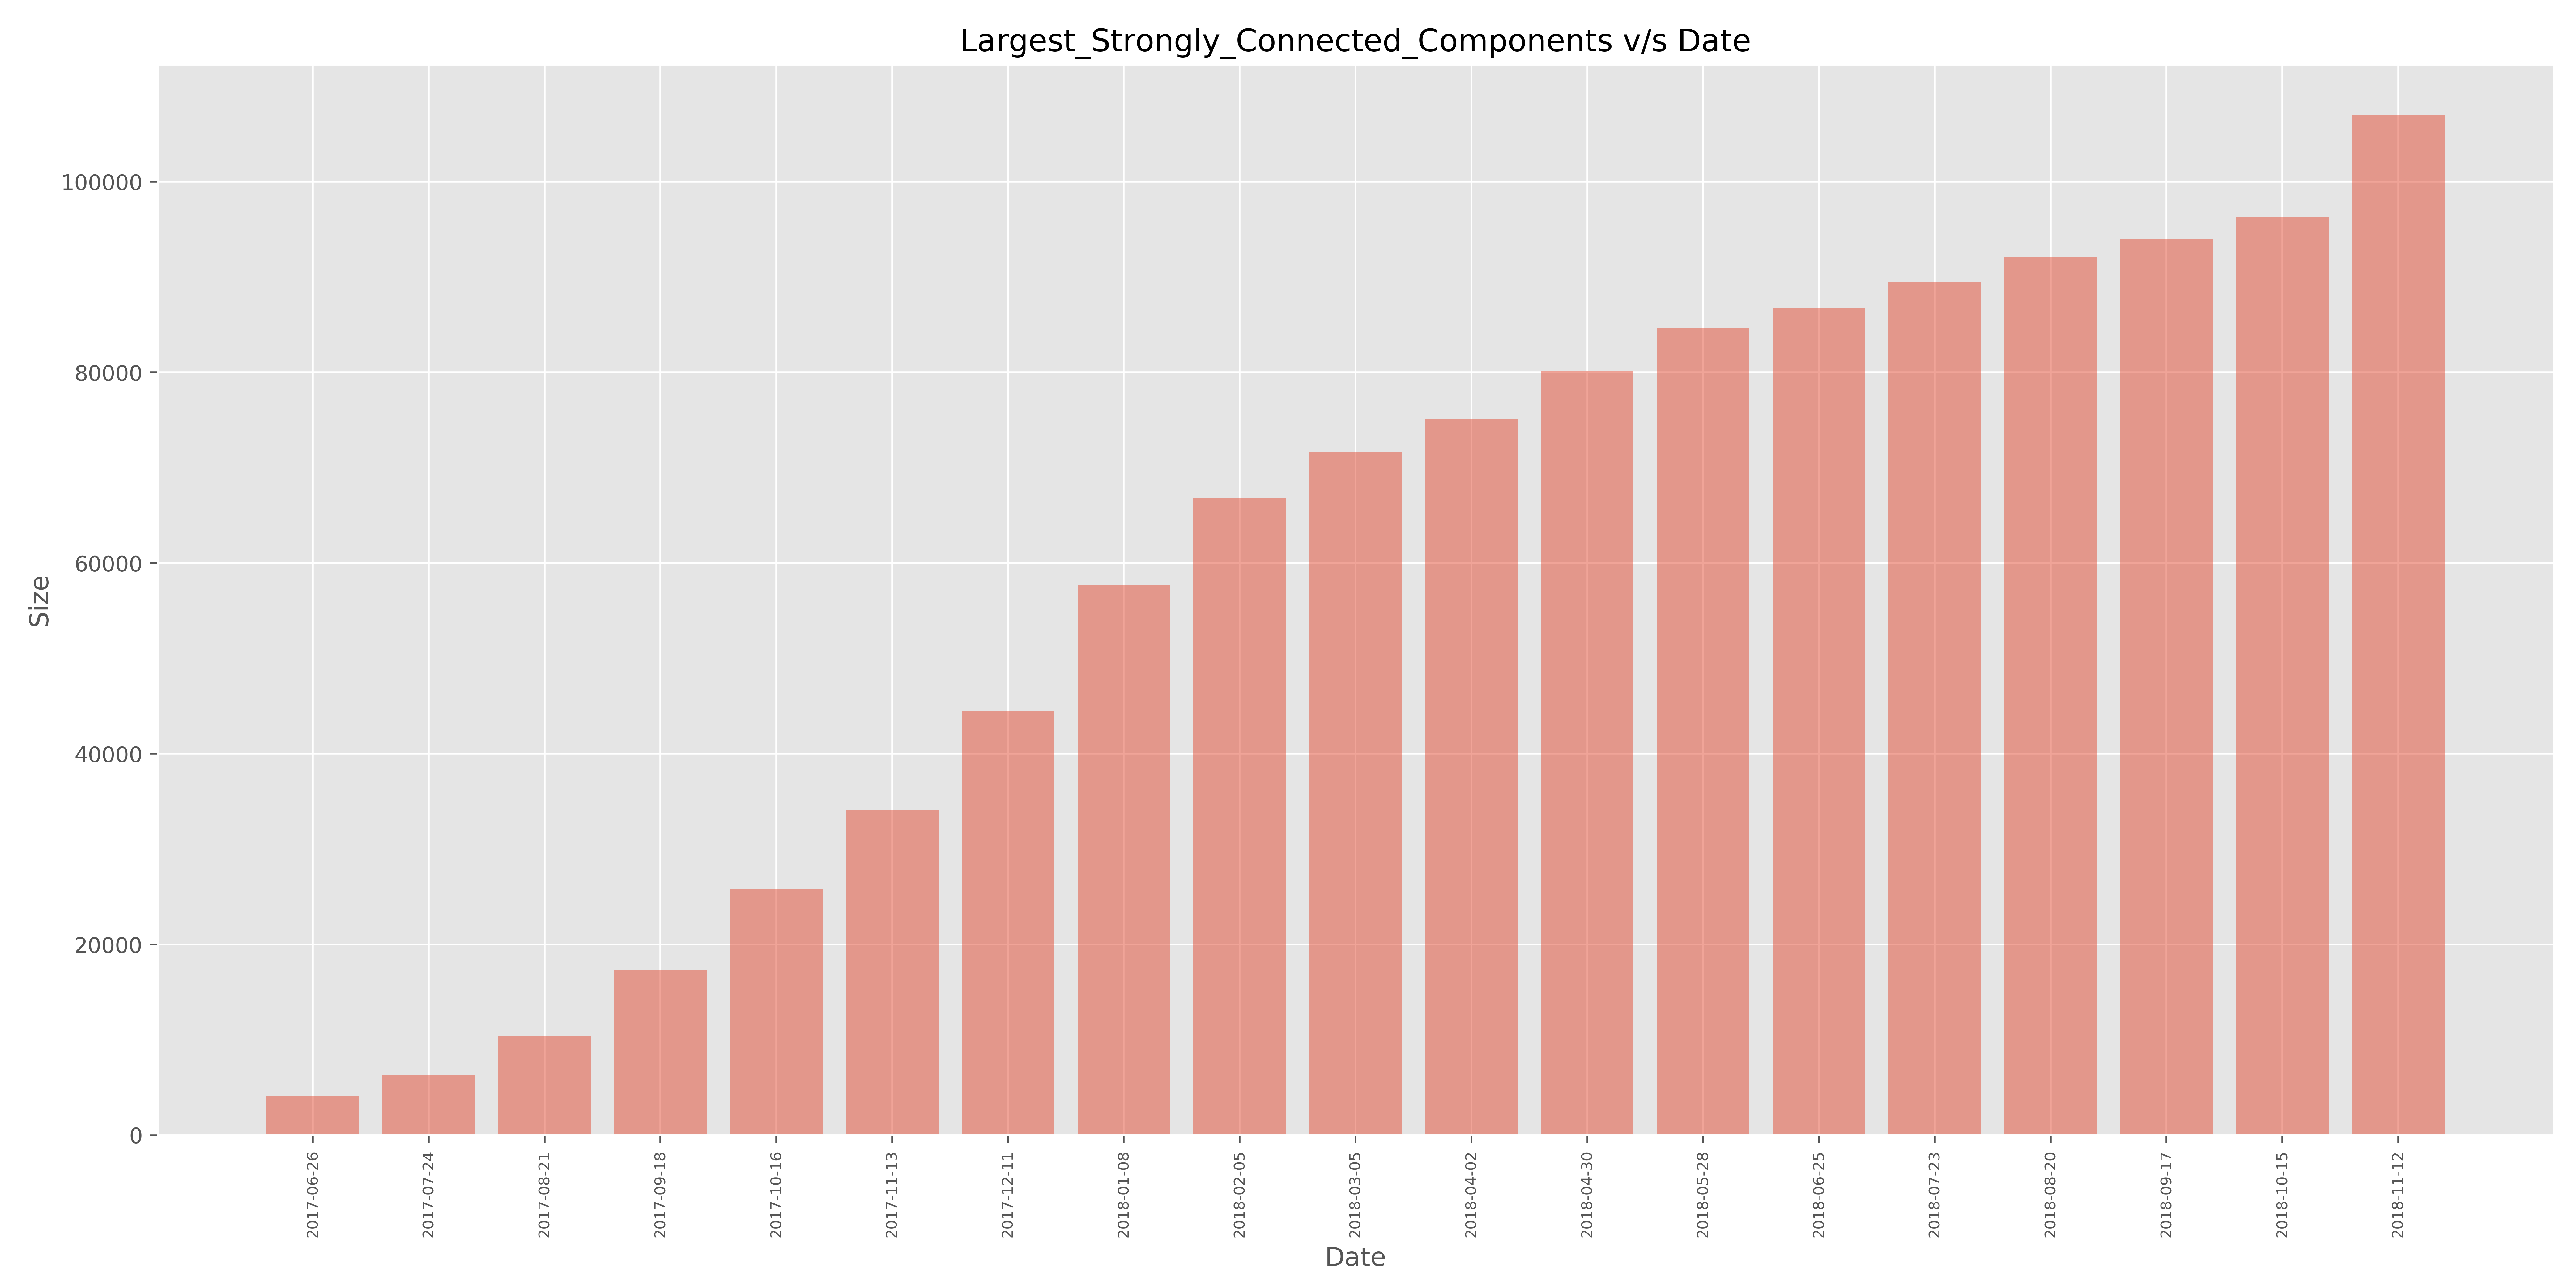
\includegraphics[scale=0.06]{Largest_Strongly_Connected_Components_vs_Date.png}
\caption{}
\label{fig:largestsccvsdate}
\end{figure*}

\begin{figure*}
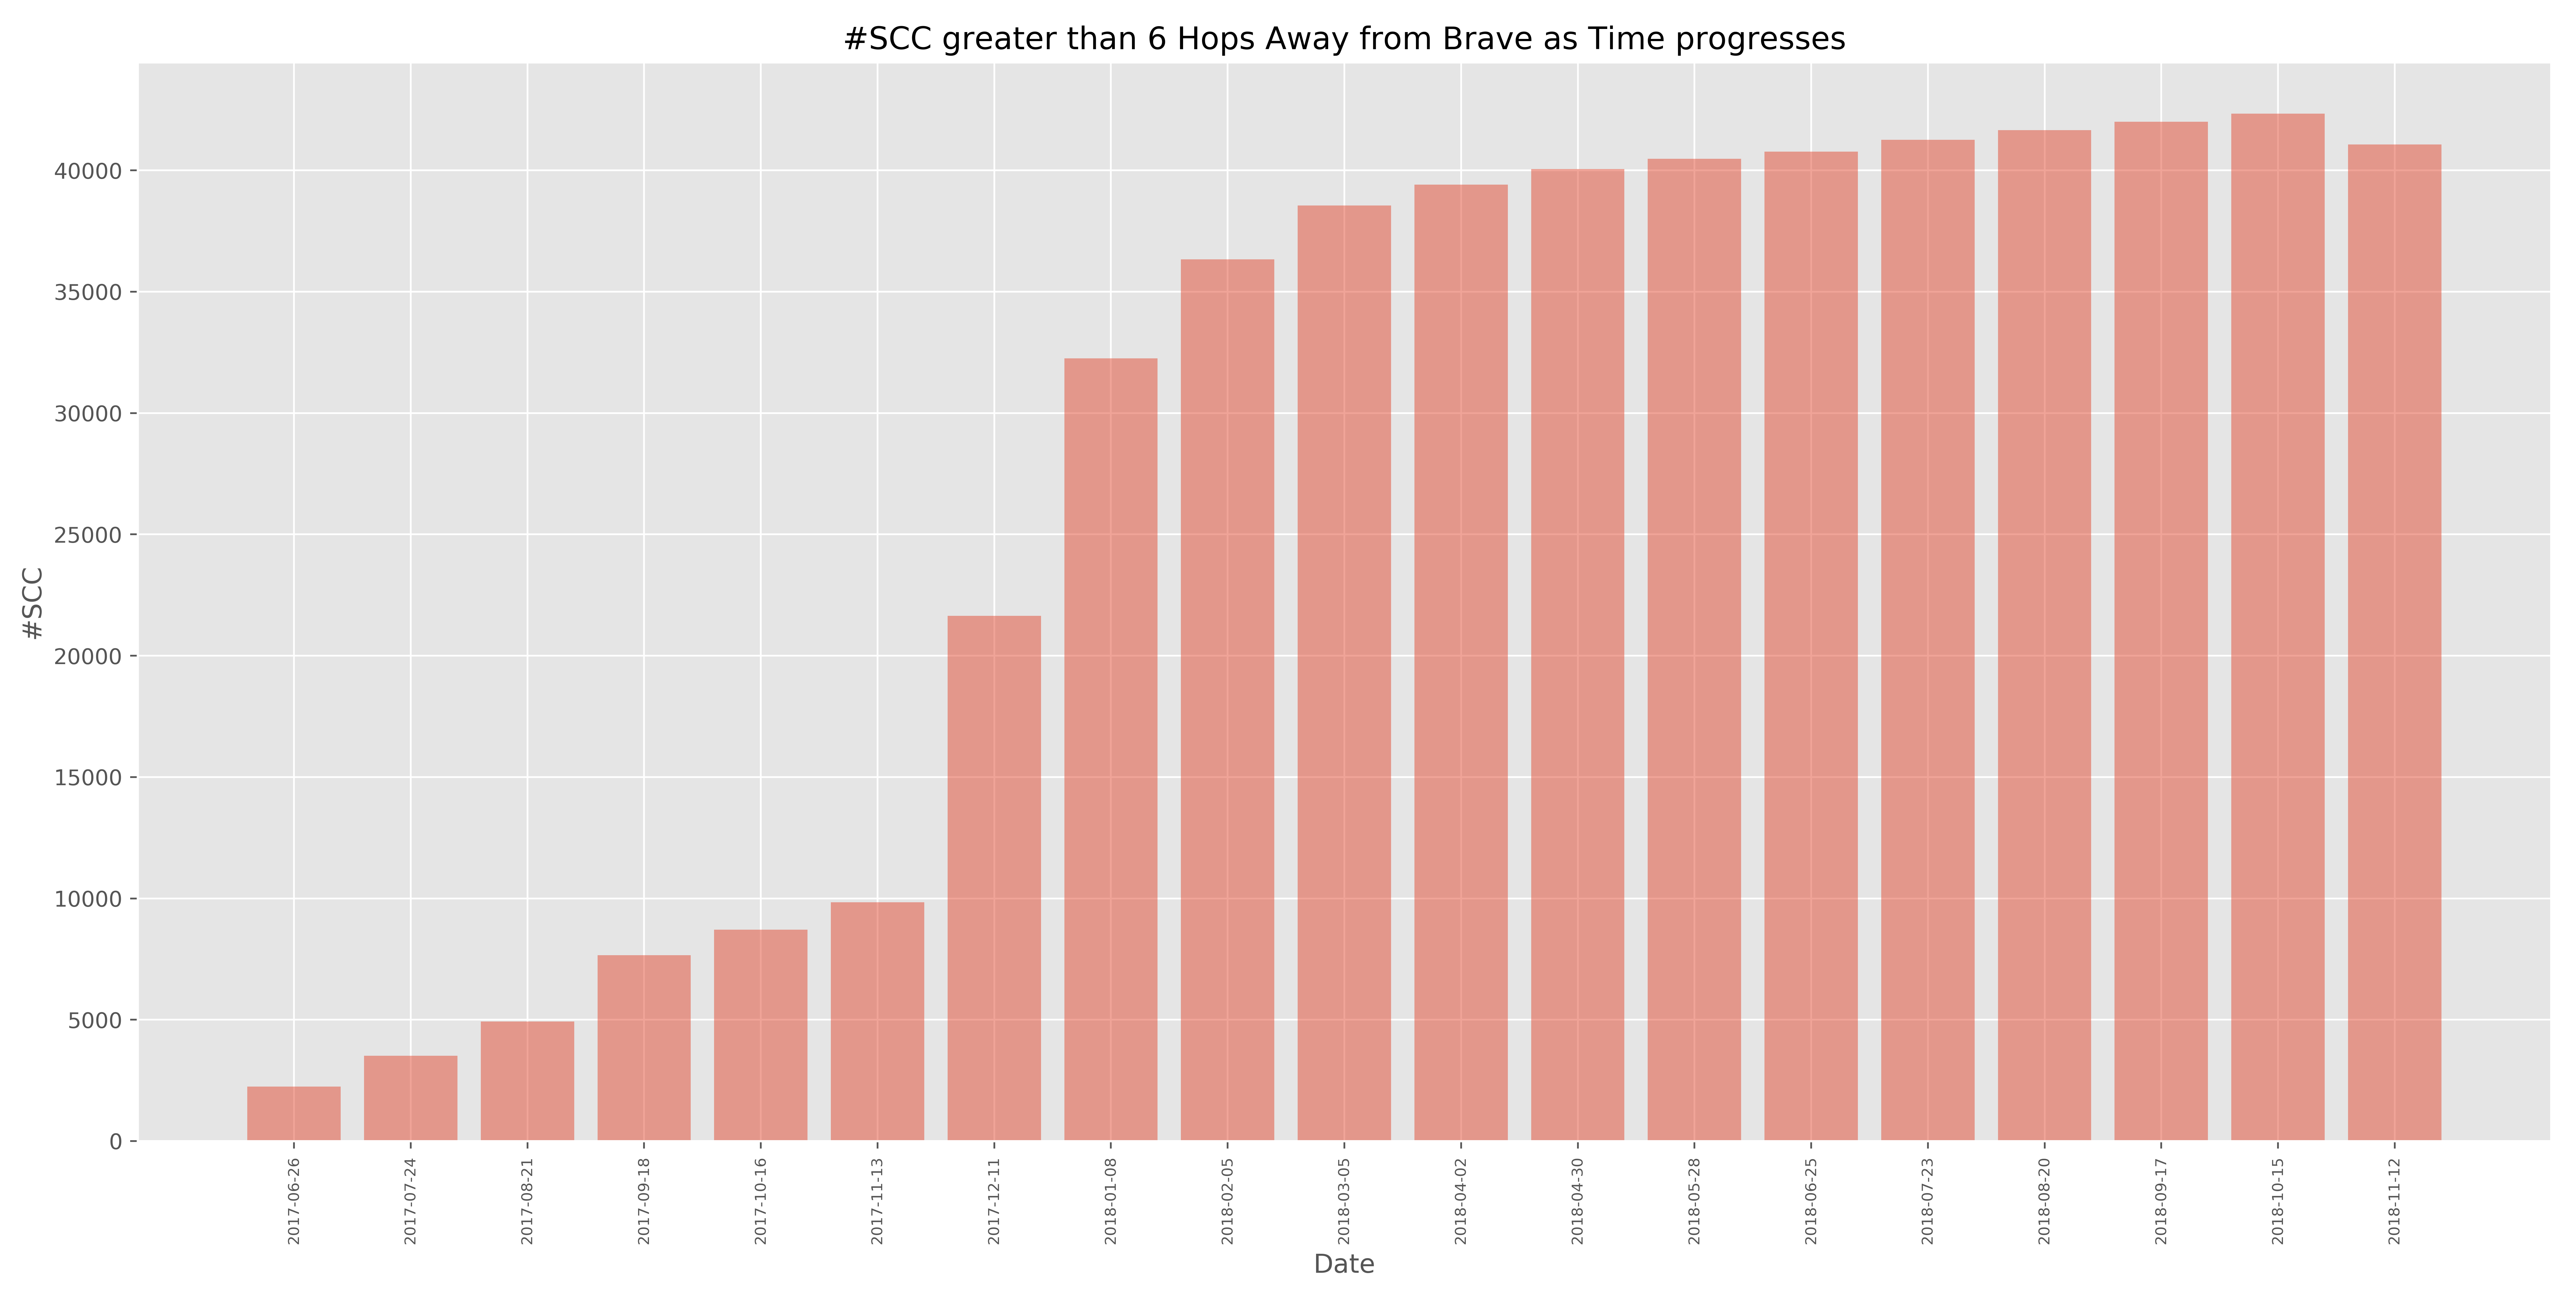
\includegraphics[scale=0.06]{SCC_greater_than_6_Hops_Away_from_Brave_as_Time_progresses.png}
\caption{ }
\label{fig:scc-hops-vs-date}
\end{figure*}

\begin{figure*}
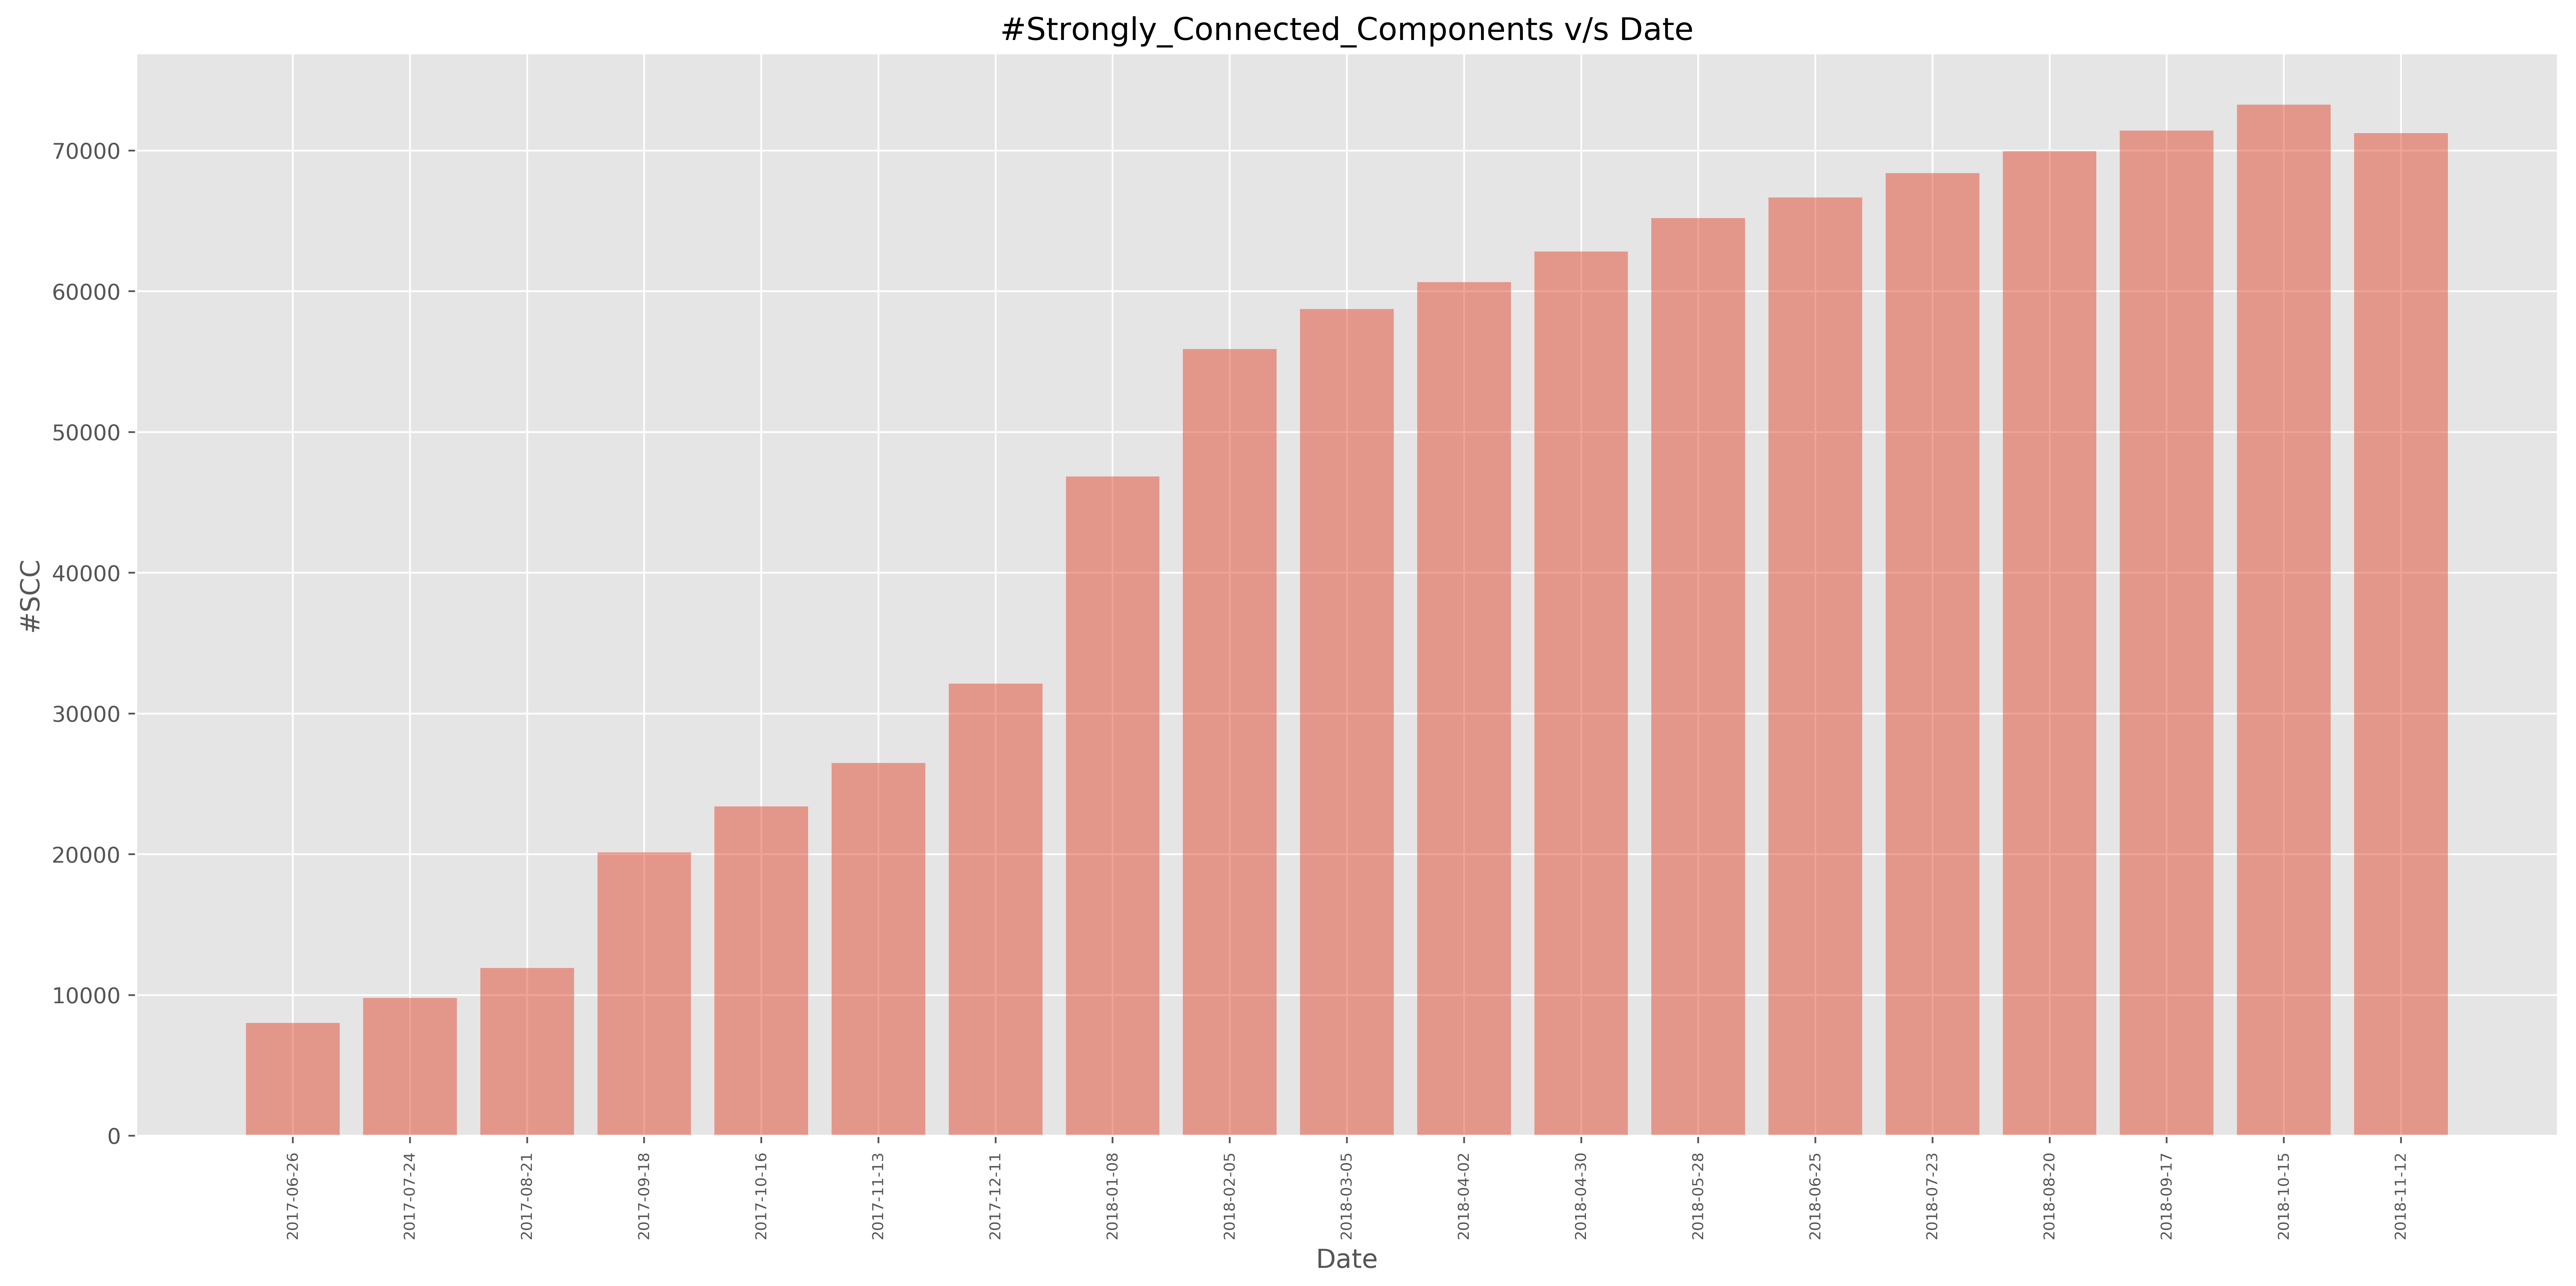
\includegraphics[scale=0.06]{Strongly_Connected_Components_vs_Date.png}
\caption{ }
\label{fig:scc-vs-date}
\end{figure*}

\begin{figure*}
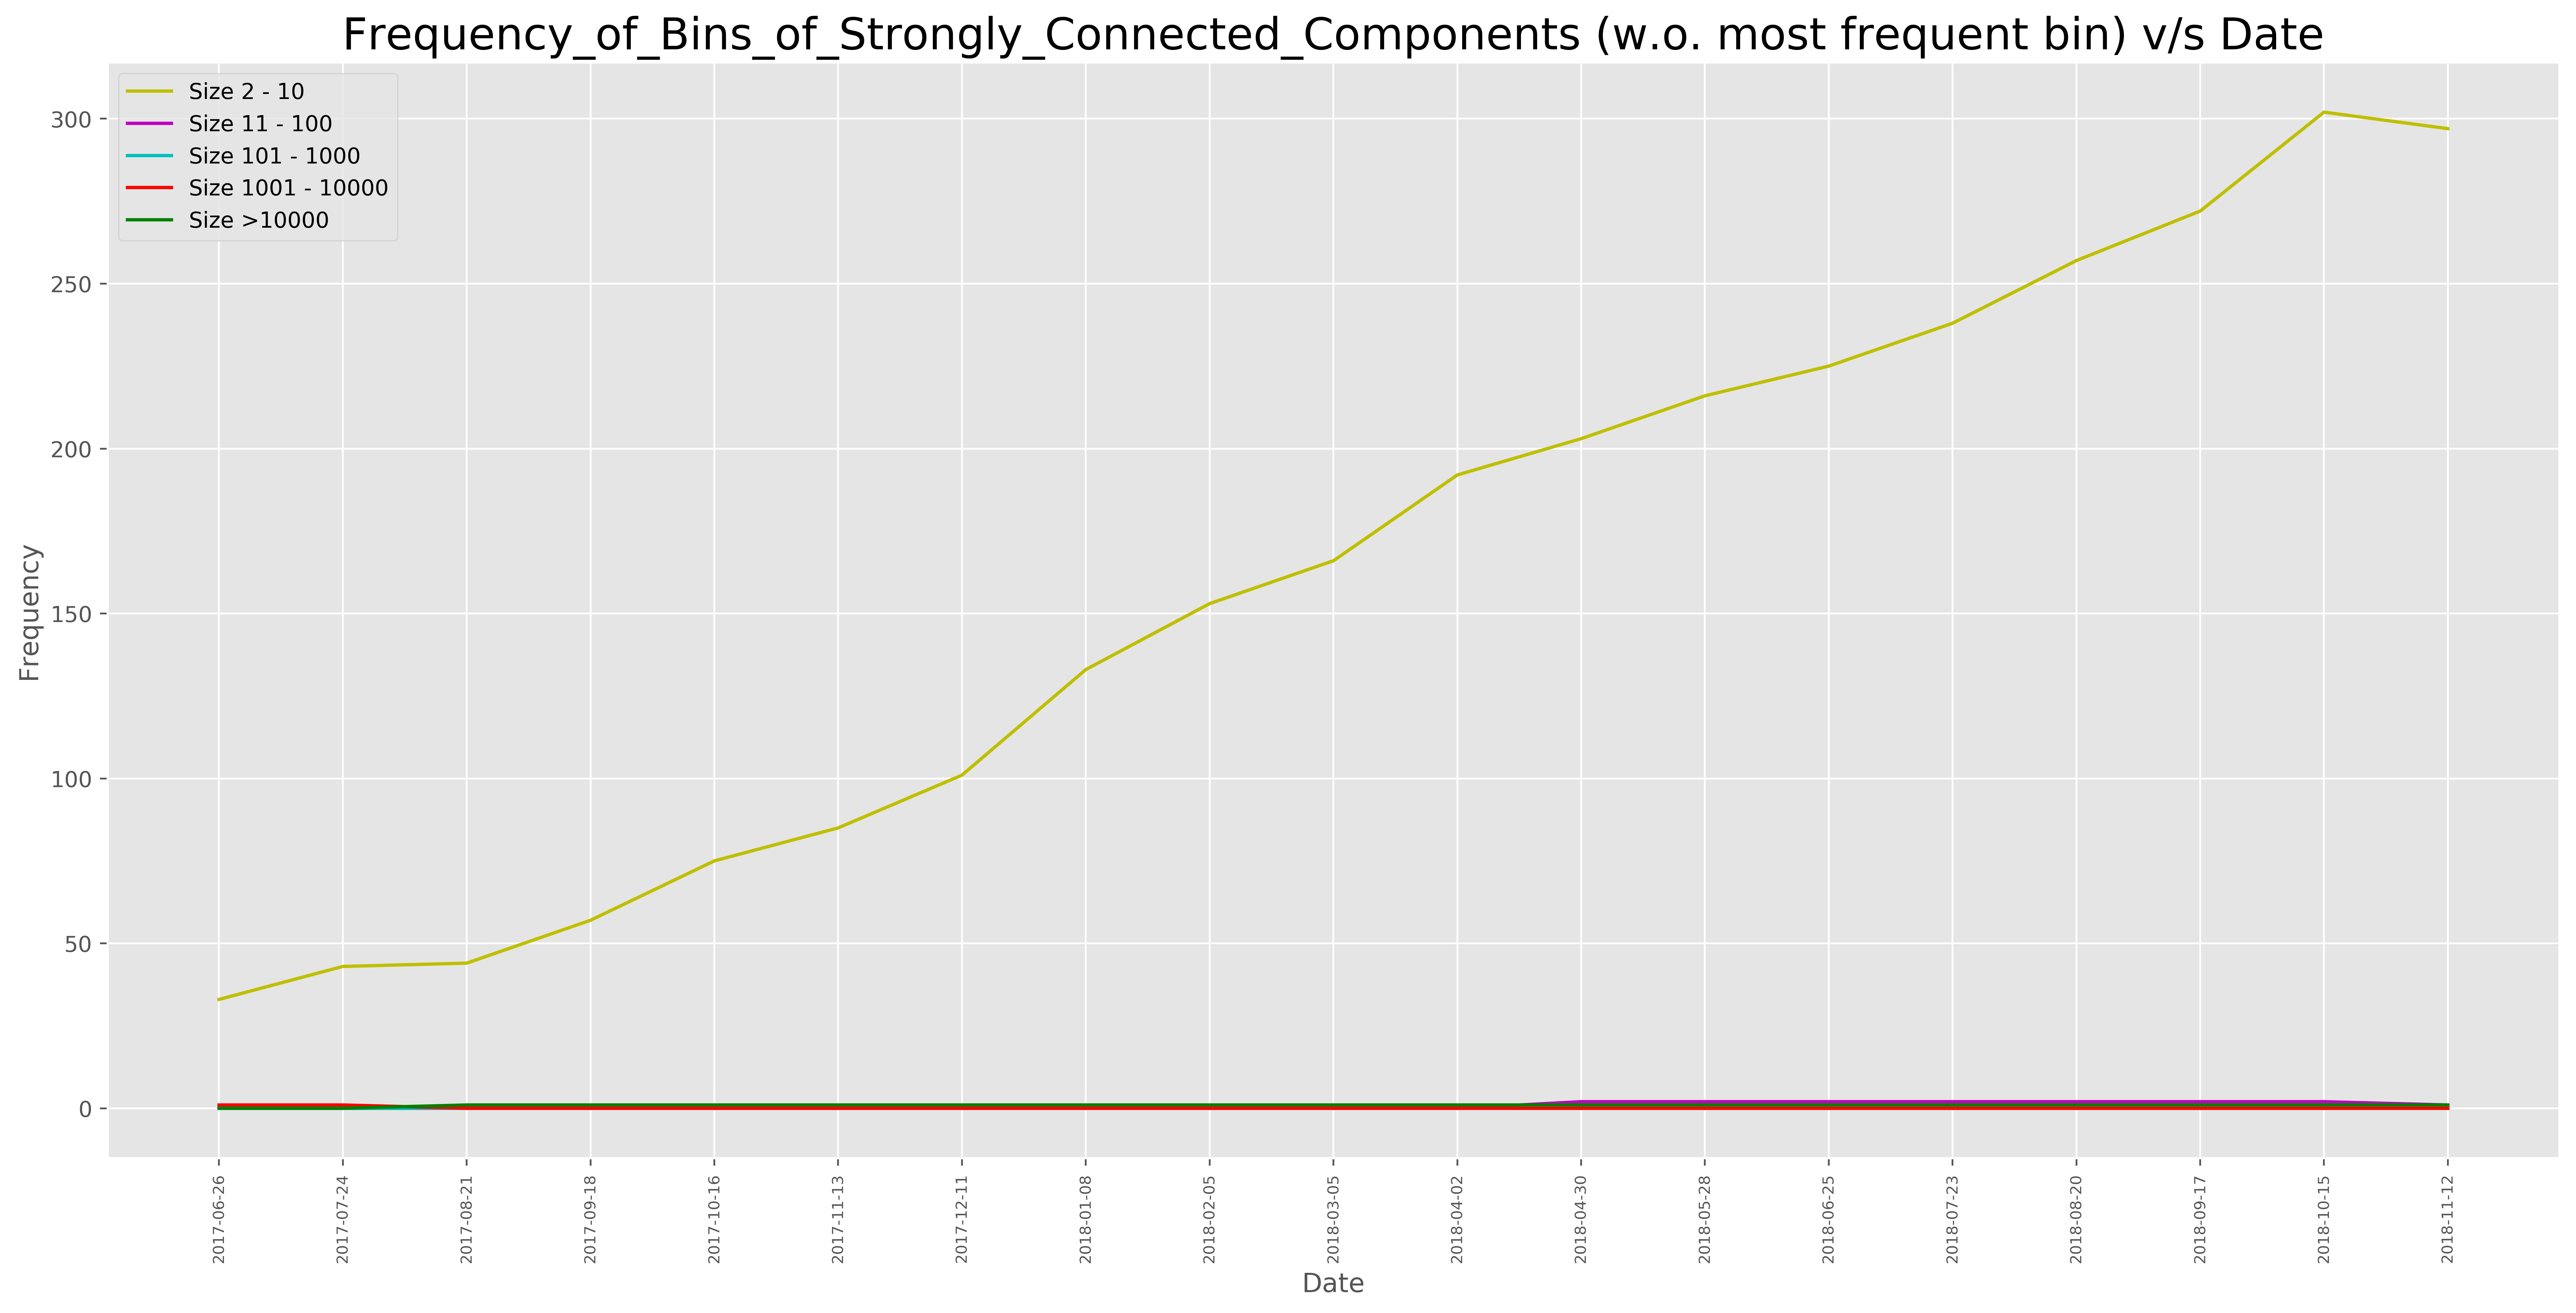
\includegraphics[scale=0.38]{Frequency_of_Bins_of_Strongly_Connected_Components_without_most_frequent_bin_vs_Date.png}
\caption{ }
\label{fig:freq-of-bins-of-scc-wo-most-freq-vs-date}
\end{figure*}

\begin{figure*}
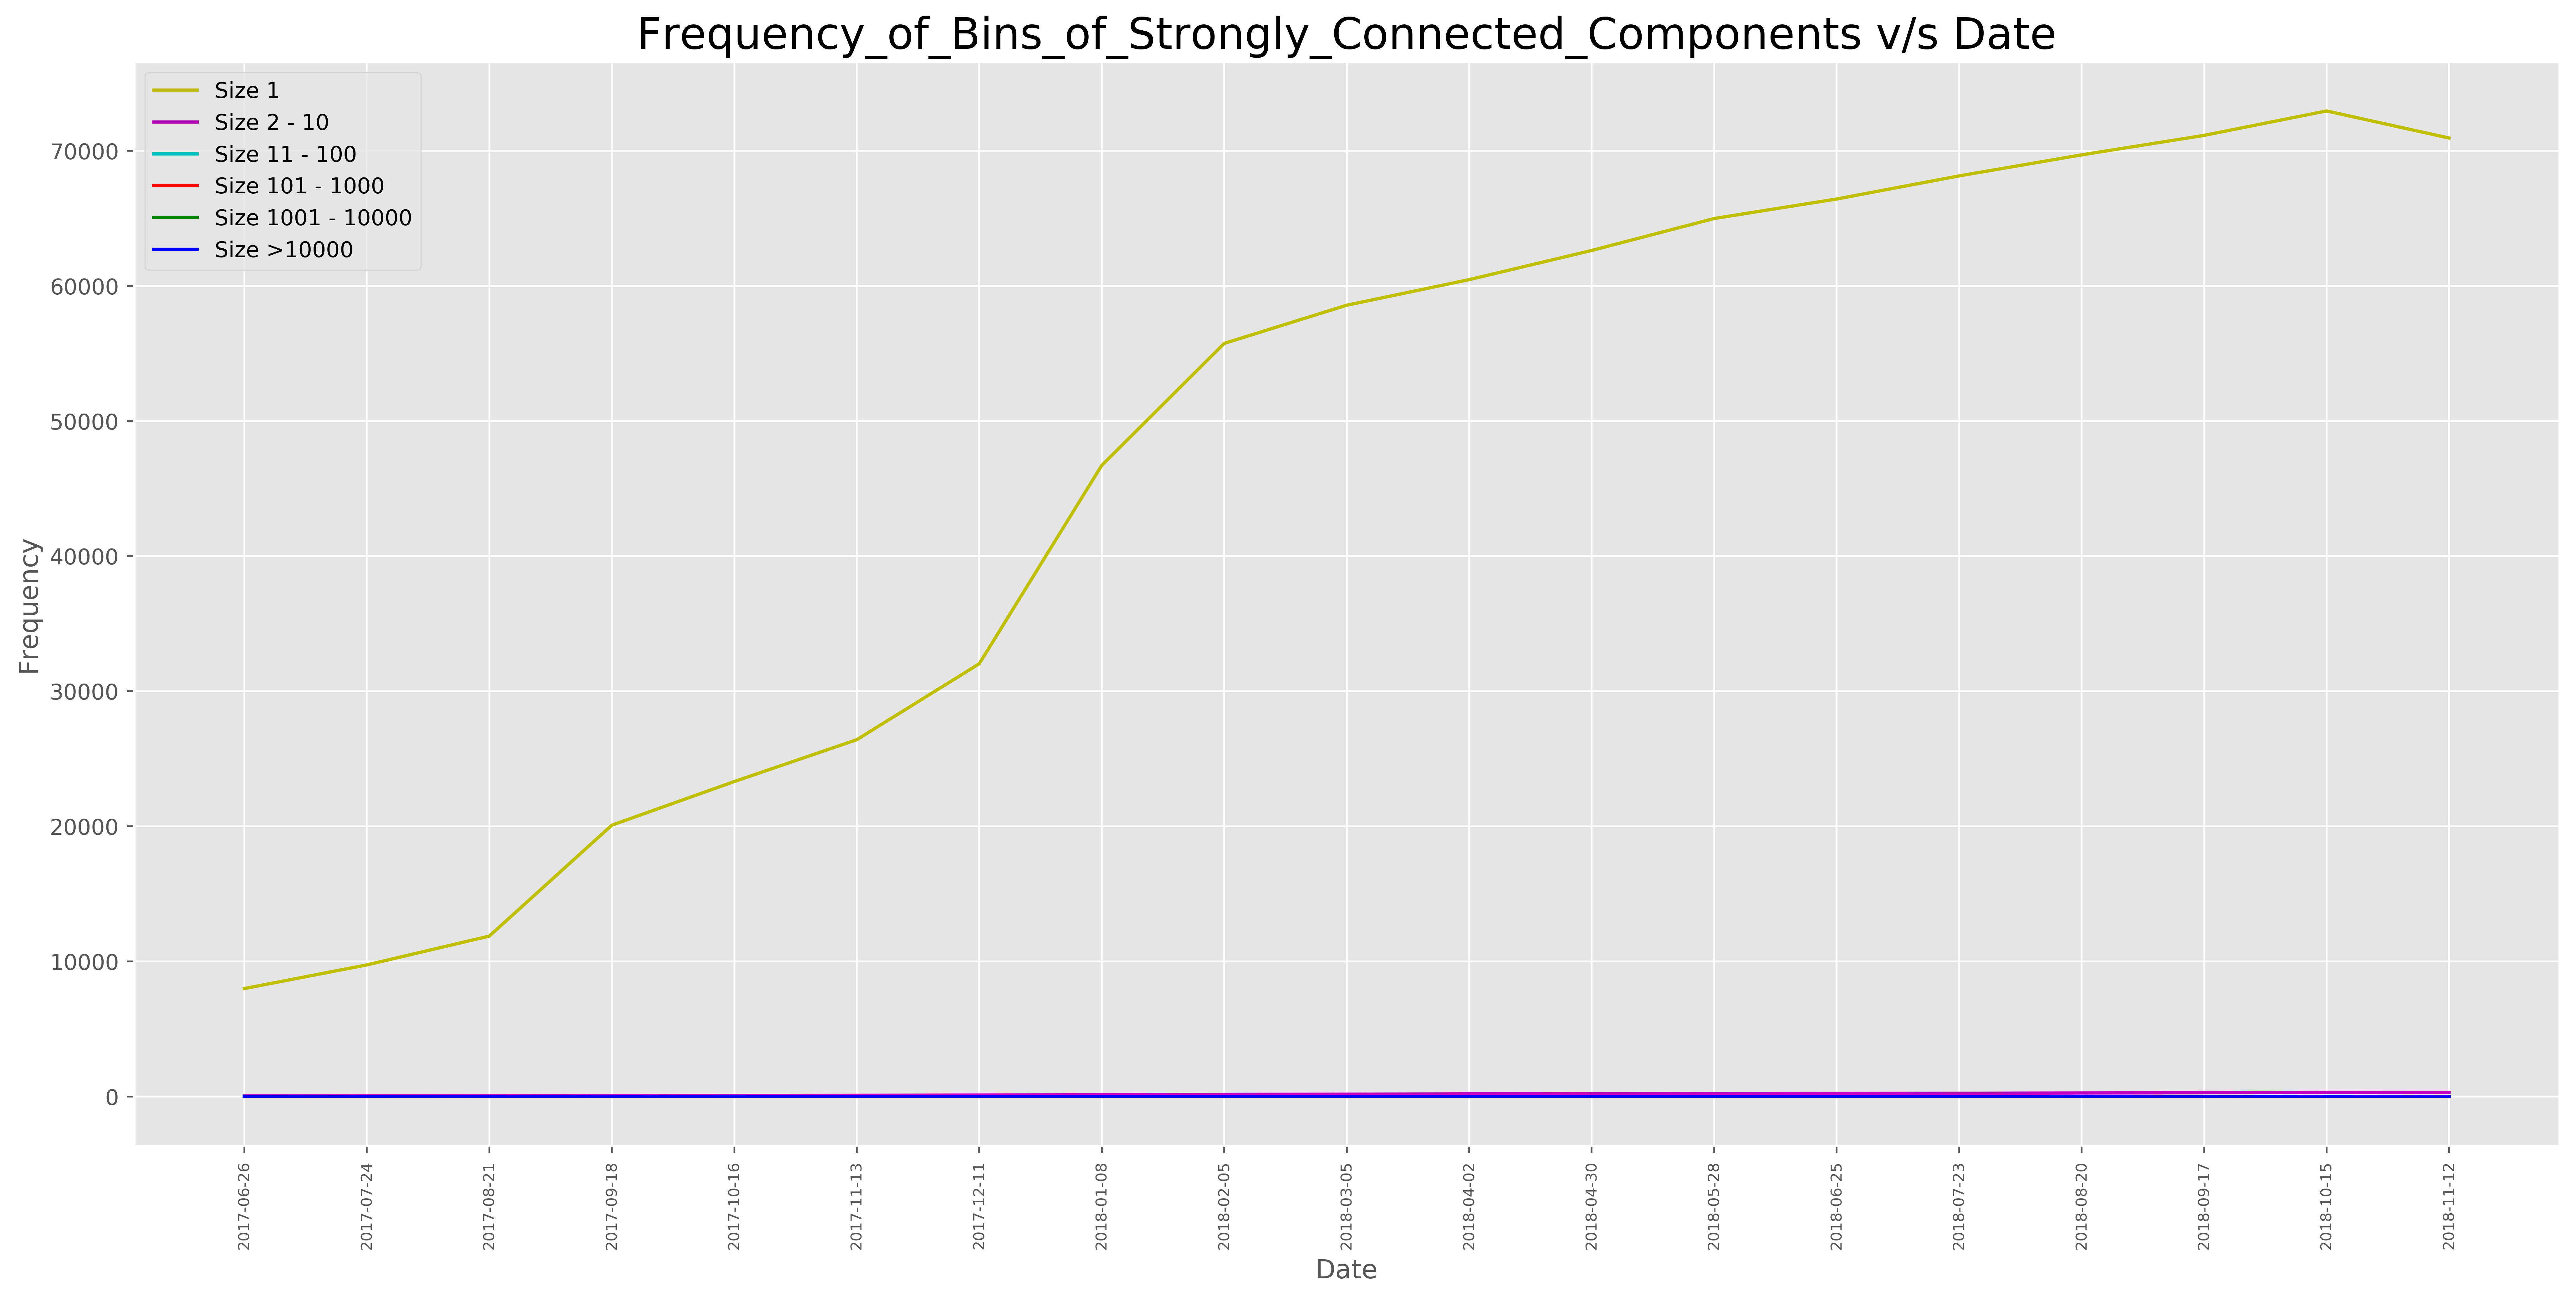
\includegraphics[scale=0.38]{Frequency_of_Bins_of_Strongly_Connected_Components_vs_Date.png}
\caption{ }
\label{fig:freq-of-bins-of-scc-vs-date}
\end{figure*}

\begin{table}[]
\begin{tabular}{|lll|}%
\hline
\bfseries ``From'' address &\bfseries \# of txs&\bfseries Total BAT \\
\hline
0x00fa6a5cb1...&1&32000000\\
0x008ed4dccc...&1&10000000\\
0x003db02d15...&1&7283200\\
\hline
\bfseries ``To'' address &\bfseries \# of txs&\bfseries Total BAT\\
\hline
0x00f948454f...&1&5000000\\
0x504433868f...&1&5000000\\
0xa82452a0b7...&1&4500000\\
0xbc84f6cdc1...&1&4000000\\
\hline
\end{tabular}
\caption{Addresses not related to Brave with large transactions}
\label{tab:non-brave-large-tx}
\end{table}

The number of Strongly Connected Components (SCCs) in the transaction
graph increases in an almost linear fashion as time progresses.
The only anomaly is the last 4 weeks where the number of SCCs decrease.
This shows that some of the SCCs fused (Figure \ref{fig:scc-vs-date}). The number of SCCs was the highest on October 15, 2018 (at around 75000).
The distribution of the sizes of SCCs is extremely skewed,
as shown in Figure \ref{fig:freq-of-bins-of-scc-vs-date}.
Most of the SCCs (around 98\%) have a size of 1
which would mean that there are many individuals who have
only transacted once.
Also, the presence of many singletons in the graph
indicates that there is some significant portion of it
has the character of a directed acyclic graph, which
contrasts with the presence of the large SCCs in the other parts of the graph.
About 2 percent of the SCC are greater than 1 but less than 6 in size (Figure \ref{fig:freq-of-bins-of-scc-wo-most-freq-vs-date}).
There is 1 large strongly connected component which consists of around 60\% of the total nodes in the graph.
Over the total time-span, this large SCC consists of about 106,000 elements (Figure \ref{fig:largestsccvsdate}).
About 50\% are less than 5 hops from the main Brave address
'0x88e2efac3d2ef957fcd82ec201a506871ad06204'\footnote{
See the ``batFundDeposit'' property at \url{https://etherscan.io/token/0x0d8775f648430679a709e98d2b0cb6250d2887ef\#readContract}.} (Figure \ref{fig:scc-hops-vs-date}).
This could hint at Brave controlling a large proportion of BAT transactions.
Additionally, there are only a few addresses which are not connected to the Brave address.
There are 487 addresses which are not a part of the BFS tree starting from the Brave address. Table \ref{tab:non-brave-large-tx} shows a list of top addresses 
from this set that have a large amount of BAT either sent or received within just a single transaction.
Additionally, it interesting to note that over the time-span of our data
a total of 125,400,000 BAT were sent from the Brave
``development pool''\footnote{See \url{https://basicattentiontoken.org/faq/\#meaning} and \url{https://etherscan.io/token/0x0d8775f648430679a709e98d2b0cb6250d2887ef?a=0x67fa2c06c9c6d4332f330e14a66bdf1873ef3d2b}.},
and a total of about 55,353,589 BAT were sent from the ``user growth pool''\footnote{See \url{https://etherscan.io/token/0x0d8775f648430679a709e98d2b0cb6250d2887ef?a=0x7c31560552170ce96c4a7b018e93cddc19dc61b6}.}.

\subsection{Brave Network Infrastructure}
\label{sec:brave_infra}
The network traffic extracted from
interactions between the Brave
browser and the Brave Software servers
indicates that currently the Brave
advertisement ecosystem centralizes
interactions between internet users and publishers.
By analyzing the publicly available source code
published on GitHub\footnote{\url{https://github.com/brave-intl/}}
by Brave, we can identify portions of code
that correspond to the HTTP request/response 
pairs recorded by Burp.
Figure \ref{fig:brave_infra} shows the high level
components revealed by the traffic analysis.
Essentially, the Brave browser represents a ``virtual''
wallet to the user, and communicates with a wallet service
to enable all of the wallet operations the user expects.
Additionally, the browser interacts with a publisher
server in order to obtain information on registered publishers.
\begin{figure}
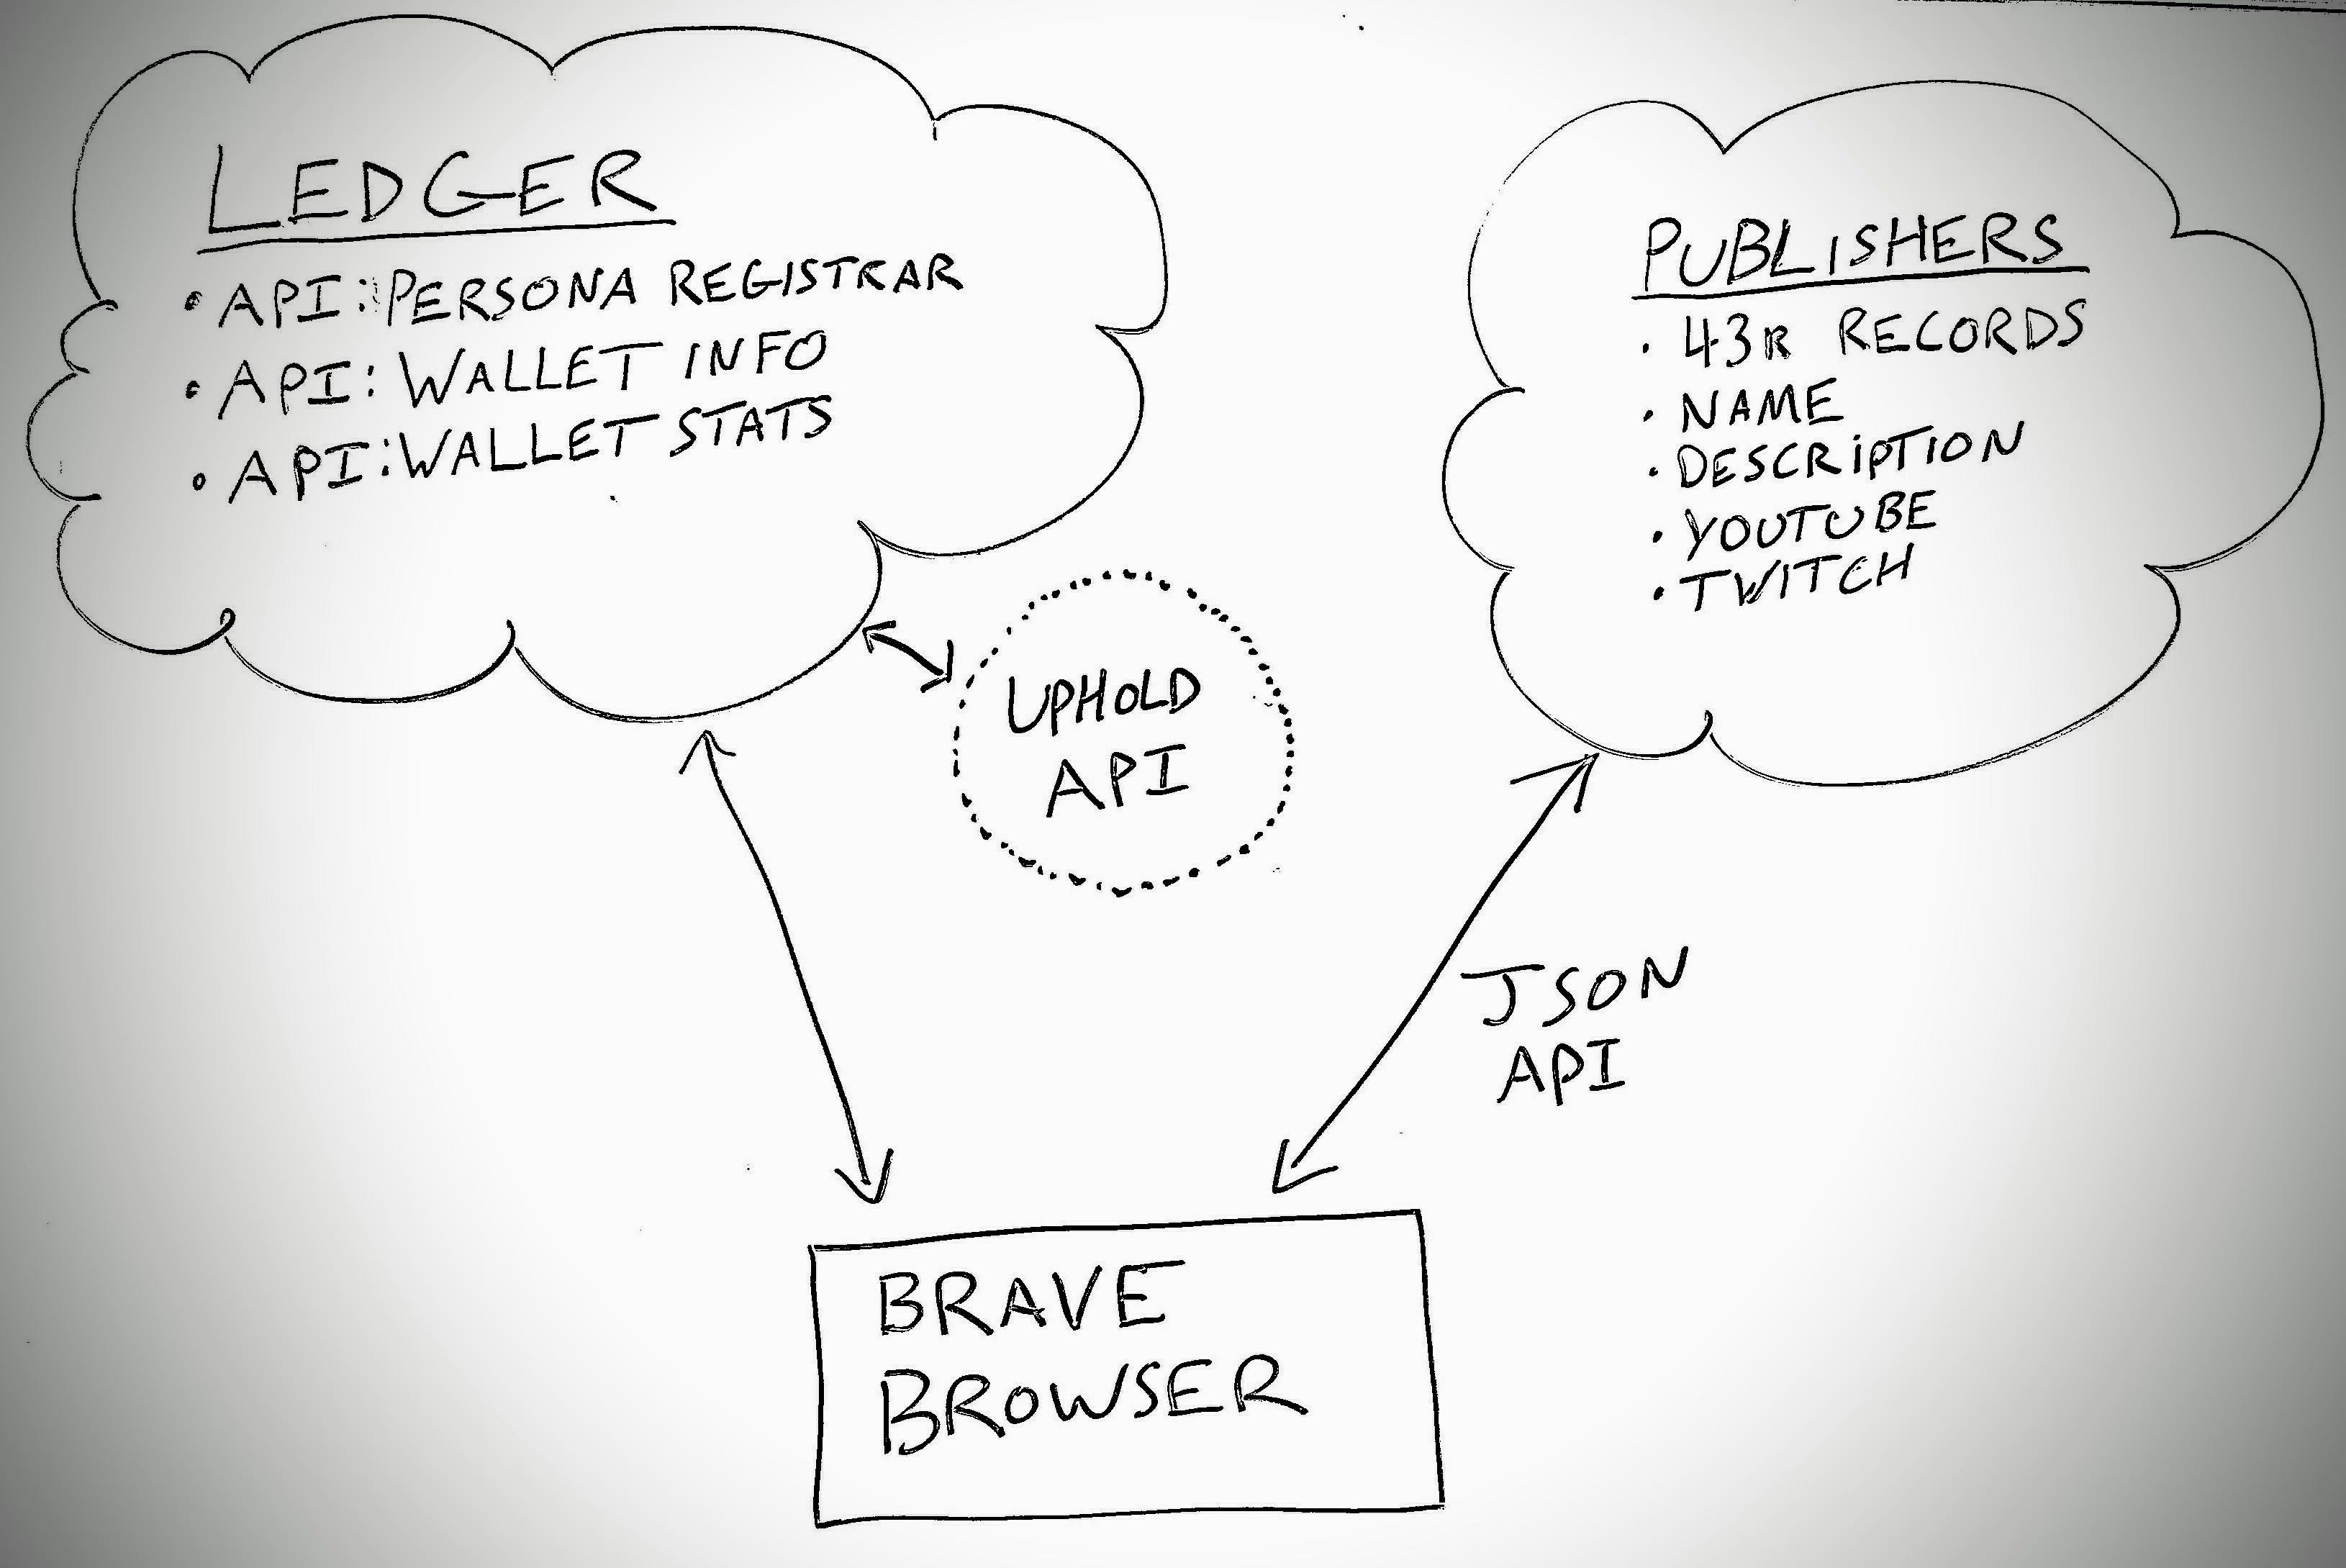
\includegraphics[scale=0.07]{brave-network-infra.jpg}
\caption{The Brave payment network infrastructure}
\label{fig:brave_infra}
\end{figure}

\subsubsection{The ``persona'' service}
Implementing BAT related user features via
a ``virtual'' wallet
allows BAT to hide many of the painful aspects of
cryptocurrencies from users. But more importantly,
Brave users never actually obtain true control of
their wallet, so therefore Brave can exercise controls
over how the user spends their BAT.
Clearly Brave must implement these kind of controls
in order to mitigate the obvious fraud related issues
relating to their frequent BAT ``giveaways''\footnote{\url{https://brave.com/brave-announces-1-million-crypto-token-giveaway/}}:
Brave facilitates every transaction related to the user wallet,
and so can therefore ensure that payments are only made to
publishers. Though most users will likely accept
restrictions like this for funds that were distributed as a ``giveaway'',
they may be less amenable to it after they start funding their
wallets themselves.
The user interface related to funding the wallet
warns the user with
\say{Reminder: The Brave Wallet is unidirectional and BAT flows to publisher sites},
so the system likely
restricts access to user sourced funds in the same way.

\begin{figure*}
\begin{lstlisting}
  std::vector<uint8_t> key_info_seed = braveledger_bat_helper::generateSeed();
  std::vector<uint8_t> secretKey = braveledger_bat_helper::getHKDF(key_info_seed);
  braveledger_bat_helper::getPublicKeyFromSeed(secretKey, publicKey, newSecretKey);
  std::string publicKeyHex = braveledger_bat_helper::uint8ToHex(publicKey);
  std::string headerDigest = "SHA-256=" + braveledger_bat_helper::getBase64(braveledger_bat_helper::getSHA256(octets));
  std::string headerSignature = braveledger_bat_helper::sign(headerKeys, headerValues, 1, "primary", newSecretKey);

  auto request_id = ledger_->LoadURL(
    braveledger_bat_helper::buildURL((std::string)REGISTER_PERSONA + "/" + ledger_->GetUserId(), PREFIX_V2),
    registerHeaders, payloadStringify, "application/json; charset=utf-8",
    ledger::URL_METHOD::POST, &handler_);
\end{lstlisting}
\caption{Select portions of ``bat\_client.cc'' related to local key initialization}
\label{fig:code_local_wallet_init}
\end{figure*}
\begin{figure*}
\begin{lstlisting}
POST /v2/registrar/persona/5e9d1759ddedd3c9a9f21c082d6071f HTTP/1.1
Host: ledger.mercury.basicattentiontoken.org

{"requestType":"httpSignature","request":{"headers":{"digest":"SHA-256=kxpeYR...","signature":"keyId=\"primary\",algorithm=\"ed25519\",headers=\"digest\",signature=\"uJzc10...\""},"body":{"currency":"BAT","label":"6176ba85-c8...","publicKey":"ba348af2..."},"octets":"{\"currency\":\"BAT\",\"label\":\"6176ba85-c8...\",\"publicKey\":\"ba348af2...\"}"},"proof":"5e9d175..."}

HTTP/1.1 200 OK
Server: Cowboy

{"wallet":{"paymentId":"83838cf4-34...","addresses":{"BAT":"0xEF192...","BTC":"1DamE...","CARD_ID":"8c36a315-2...","ETH":"0xEF192...","LTC":"LcoVE..."}},"payload":{"adFree":{"currency":"BAT","fee":{"BAT":25},"choices":{"BAT":[15,20,25,30,50,100]},"range":{"BAT":[15,100]},"days":30}},"verification":"6x+vmW..."}
\end{lstlisting}
\caption{POST request to register a new ``persona'' within the Brave payment system}
\label{fig:post_persona}
\end{figure*}

Figure \ref{fig:code_local_wallet_init} shows that
upon starting up for the first time, the Brave browser will generate
an asymmetric keypair and then make a request to
``ledger.mercury.basicattentiontoken.org''\footnote{See \url{https://github.com/brave-intl/bat-native-ledger/blob/f72aad5f4e85a50980ee657b51da3df054db0b47/src/bat_client.cc}, line 80 for the full code.}.
The HTTP POST request/response shown in Figure \ref{fig:post_persona}
shows an example of the data that the browser sends, and the
data sent back by the server. This example response indicates
that a new account (or ``persona'') has been registered,
and the Brave browser will henceforth use ``paymentId'' field
as a reference for its wallet. The corresponding server
code shown in Figure \ref{fig:code_uphold_persona_register}
verifies the received parameters, generates a new UUID
to represent this new wallet, and then creates an entry
in the wallet database\footnote{See
\url{https://github.com/brave-intl/bat-ledger/blob/08cda19f4c7972764c2bf9b6408fcb19acae2cbc/ledger/controllers/registrar.js} line 125 for the full code.}.
Finally, observe that the code (shown in Figure \ref{fig:code_uphold_wallet_create})
that corresponds
to the call to function ``runtime.wallet.create''
(in the ``createPersona'' function)
simply delegates to several invocations
of the Uphold API for creating ``cards''
\footnote{See \url{https://github.com/brave-intl/bat-ledger/blob/26913b9137a006f0c9bc77d75a13ded878935b9c/bat-utils/lib/runtime-wallet.js} line 277.}.

\begin{figure}
\begin{lstlisting}
const createPersona = function (runtime) {
<...>
    const uId = request.params.uId.toLowerCase()
    const proof = request.payload.proof
    registrar = runtime.registrars['persona']
<...>
    const paymentId = uuid.v4().toLowerCase()
    const wallets = runtime.database.get('wallets', debug)
<...>
    try {
      result = await runtime.wallet.create(requestType, requestBody)
<...>
  }
}
\end{lstlisting}
\caption{Code to create persona}
\label{fig:code_uphold_persona_register}
\end{figure}

\begin{figure}
\begin{lstlisting}
Wallet.providers.uphold = {
<...>
  create: async function (requestType, request) {
<...>
        try {
          wallet = await this.uphold.api('/me/cards', { body: request.octets, method: 'post', headers: request.headers })
          ethAddr = await this.uphold.createCardAddress(wallet.id, 'ethereum')
          btcAddr = await this.uphold.createCardAddress(wallet.id, 'bitcoin')
          ltcAddr = await this.uphold.createCardAddress(wallet.id, 'litecoin')
\end{lstlisting}
\caption{Code to create Uphold payment instruments via the Uphold API}
\label{fig:code_uphold_wallet_create}
\end{figure}
According to its founder,
Uphold is a payment company that
aims to
\say{make it easy and frictionless for anyone, anywhere to move, convert, hold and transact in any form of money or commodity securely, instantly and for free}\cite{fortune-uphold}.
According to the sign-up page\footnote{\url{https://uphold.com/en/how-it-works/membership}},
a user can fund their account via a cryptocurrency
or a bank account and also can withdraw to a bank account,
though it doesn't appear that Uphold intends to
provide ``trading'' type services like many other
companies involved in cryptocurrency.
The OAuth 2.0 compliant Uphold API\footnote{See \url{https://uphold.com/en/developer/api/documentation/\#authentication} and \url{https://uphold.com/en/developer/api}}
allows third parties to read, modify, and transact with
Uphold accounts. In particular a third party
can create a ``card'' object\footnote{See \url{https://uphold.com/en/developer/api/documentation/\#card-object}}
denominated in a cryptocurrency, such as BAT, Ethereum, or Bitcoin.
The code in Figure \ref{fig:code_uphold_wallet_create}
utilizes the Uphold Javascript API\footnote{See \url{https://uphold.github.io/uphold-sdk-javascript/actions/card-address/create-card-address.html}}
to create new ``card'' objects associated with the User's
Uphold wallet.
Brave's interaction with the Uphold API in this manner is
consistent with some of their public announcements\footnote{See \url{https://basicattentiontoken.org/uphold-to-support-braves-basic-attention-token-the-new-utility-token-for-blockchain-based-digital-advertising/}}
and with the information displayed by some parts
of the Brave browser user interface.
For example, Figure \ref{fig:brave_uphold_wallet} shows a screenshot of the 
Brave rewards interface in the Brave browser,
wherein the UI indicates that the user's wallet
is ``managed'' by Uphold.

\begin{figure}
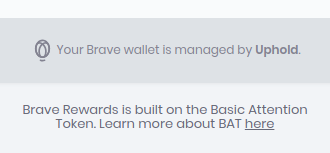
\includegraphics[scale=0.5]{wallet-managed-by-uphold-screenshot.png}
\caption{A screenshot of the ``Brave Rewards'' UI of the Brave browser}
\label{fig:brave_uphold_wallet}
\end{figure}

Finally, a number of other interesting API requests to
the ledger server are shown in Appendix \ref{app:addition_brave_api_stuff}.
These include an endpoint to translate the public key part of
the local keypair into the payment ID (see Figure \ref{fig:get_pk2PID}),
an endpoint to obtain the balance of the wallet
associated with a payment ID (along with some other miscellaneous info; see Figure \ref{fig:get_PID2wallet}),
and two HTTP logs that show how the browser queries for/obtains
free BAT when a ``giveaway'' promotion is active
(Figures \ref{fig:get_grant} and \ref{fig:put_grant}).

\subsubsection{The publisher API server}
In addition to the ``ledger'' server,
we also obtained network traffic of note that was going to/from the 
domain publishers.basicattentiontoken.org.
Figure \ref{fig:pubs_routes} shows the Ruby-on-Rails routes\footnote{See line 96 of \url{https://github.com/brave-intl/publishers/blob/7dccb26d4f05e9497bcebe1e0ac55b321a75f880/config/routes.rb}}
in their published code 
on GitHub, in which the the ``/api/v1/public/channels'' path
occurs. This path is the only public/non-authenticated
endpoint of the publisher service
that we were able to confirm. We observed that upon
startup, the Brave browser makes a GET request to this
API controller in order to obtain a list of publisher information.
Figure \ref{fig:get_pubs} shows a selected portion
of one of these request/response pairs.

\begin{figure}
\begin{lstlisting}
# /api/v1/stats/
namespace :stats, defaults: { format: :json } do
  namespace :channels, defaults: { format: :json } do
    get :twitch_channels_by_view_count
    get :youtube_channels_by_view_count
...
    get :javascript_enabled_usage
  end
end
# /api/v1/public/
namespace :public, defaults: { format: :json } do
  get "channels", controller: "channels"
end
\end{lstlisting}
\caption{possible API endpoints for the ``publisher'' service}
\label{fig:pubs_routes}
\end{figure}

\begin{figure}
\begin{lstlisting}
GET /api/v1/public/channels HTTP/1.1
Host: publishers.basicattentiontoken.org

HTTP/1.1 200 OK
Server: Cowboy
Date: Mon, 26 Nov 2018 01:02:00 GMT
...
Content-Length: 2444055

[["heliat.fr",true,false,{}],...["chainshuttle.com",true,false,{"title":"Hi Brave user!","description":"If you would like to support Chainshuttle you can leave a tip.","backgroundUrl":null,"logoUrl":null,"donationAmounts":[1,5,10],"socialLinks":{"youtube":"","twitter":"","twitch":""}}],["lastend.com",true,false,{}],...
\end{lstlisting}
\caption{GET request to obtain the list of registered Brave publishers}
\label{fig:get_pubs}
\end{figure}

As part of its primary functionality,
the Brave browser must recognize a publisher
website, present publisher information to the user,
and communicate details about the user's
selection of publishers to support via payments.
Because it must implement this functionality,
it is likely that the data found in the JSON file
served by the ``channels'' controller represents the 
current state of the Brave publisher registry.
Obviously the first field of an element of
this data determines the name of the publisher,
and the fourth element represents some
descriptive data meant for the benefit of the user.
Figure \ref{fig:pub_json_decode} shows a small snippet
of a helper file\footnote{See line 1880 in \url{https://github.com/brave-intl/bat-native-ledger/blob/f72aad5f4e85a50980ee657b51da3df054db0b47/src/bat\_helper.cc}.}
of the browser source code that is
related to decoding the publisher JSON file.
The variable names indicate that the second and third
fields determine some kind of ``verification''
and ``exclusion'' status of a publisher.
The verification status likely relates to the 
verification procedure required by Brave as part of the 
registration procedure\footnote{See \url{https://brave.com/faq-rewards/\#verified-publishers}.}.
On the other hand, the exclusion list seems to have something to
do with the default payment behavior of the Brave browser
with respect to a selection of website, as hinted by
a comment in a configuration\footnote{See \url{https://github.com/brave-intl/publishers/blob/9010d4774abbf822eb49db72f9d01d2551c43aeb/config/excluded\_site\_channels.yml}} file of the publisher service
source code:
\say{A list of site channels which are not included in browser contributions by default.
The general rule of thumb is that we try to not auto-pay sites that users already pay,
such as commerce sites, financial services sites like banks, SaaS vendors and government sites}.

\begin{figure}
\begin{lstlisting}
item.verified = i[1].GetBool();
item.excluded = i[2].GetBool();
\end{lstlisting}
\caption{Code for decoding the JSON file from the publisher service}
\label{fig:pub_json_decode}
\end{figure}
Table \ref{fig:pub_json_stats} shows some basic data regarding
43115 entries in the publisher registry.
The most interesting data here is that only two thirds
of the registered publishers have completed
the verification process.
Additionally, most publishers have not bothered to
create any description of themselves, and only
a small minority of Twitch and YouTube publishers
are both verified and have a description.

\begin{table}[]
\begin{tabular}{|lll|}
\hline
Type & Count & Proportion \\
\hline
Verified & 28605& 66.3\% \\
Unverified & 14510 & 33.7\% \\
Excluded & 14526& 33.7\% \\
Has banner data & 1457& 3.4\% \\
YouTube & 18835& 43.7\% \\
Twitch & 1674& 3.9\% \\
YouTube: verified \& banner & 683& 3.6\% (of YouTube) \\
Twitch: verified \& banner  Publishers & 130& 7.8\% (of Twitch) \\
\hline
\end{tabular}
\caption{Breakdown of publisher registry data}
\label{fig:pub_json_stats}
\end{table}


\section{Conclusion}
The current Brave payment ecosystem does not currently exhibit the 
type of decentralized structure that smart contracts invite.
Our analysis in Section \ref{sec:brave_infra} supports a
hypothesis that Brave centralizes the interactions between
users and publishers within their own network infrastructure,
and manage the funds involved via the Uphold API.
This hypothesis is explicitly confirmed to some extent by
members of the BAT team on the currency's
official subreddit\footnote{See \url{https://www.reddit.com/r/BATProject/comments/a04wo7/why\_does\_my\_bat\_wallet\_have\_no\_transactions/}.}, as they state that transactions between
publishers and users happen off-chain.
Further, they confirm that user sourced funds sent to a wallet
via the ``Add Funds'' feature of the browser are moved into
a pool of funds within Uphold and controlled by BAT.
The centralization of the current payment network in some sense
conflicts with the manifestation of the BAT token as a cryptocurrency:
why is it that Brave needed to have an ICO and implement BAT as a token?
For a centralized payment system in which all users and all publishers
must pass through Brave infrastructure to interact, they could have
implemented it in a much simpler way. For example, they could
work with a payment processing company like Stripe, then
have a payment UI in their browser which enables the user to make
a deposit (say, several dollars), and then Brave can make
micropayments to registered publisher accounts. None of this
requires a cryptocurrency, and yet it provides the same security and
anonymity. This means that at the moment, the only benefit Brave
is obtaining from having created BAT is 1) the hype of cryptocurrency
ICO funding, and 2) not having to deal with traditional payment
processors for users to join. Of course, for 2) they still
had to collaborate with some kind of payment processor: Uphold.
As a part of data collection efforts the authors attempted to
go through the ``Add funds'' procedure within the Brave browser
UI. This required several time consuming steps.
First, we had to register an Uphold account, which
requires more detailed personal information than just a credit card,
such as a scan of a passport, visa, or drivers license, and
also involves an ``identity verification'' waiting period.
Second, we had to fund the account with a credit card or a
bank account. These two steps are already less convenient than
simply providing a credit card directly to a traditional payment processor.
However, what's worse is that we were unable to successfully fund our Uphold account
even after trying three different credit cards and a bank account:
in each case Uphold gave a cryptic error.
Given the difficulties that we encountered attempting to join this ecosystem,
we believe that is is unlikely that a large number of Brave users
have funded their wallets with any funds beyond that which was
gifted to them by Brave. In this sense,
it is arguable that Brave's
use of a cryptocurrency to enable payments to publishers seems
counterproductive to adoption, though it was clearly
beneficial to funding the development of the system.

\bibliographystyle{ACM-Reference-Format}
\bibliography{bibliography}

\begin{appendices}
\section{Additional Brave API requests/responses}
\label{app:addition_brave_api_stuff}
\begin{figure*}
\begin{lstlisting}
GET /v2/wallet?publicKey=ba348af260222c5c3ea2d97d72a5813ab610640a1f16db734b56842e70cd6417 HTTP/1.1
Host: ledger.mercury.basicattentiontoken.org

HTTP/1.1 200 OK
Server: Cowboy

{"paymentId":"ec30a106-addb-42dd-9c61-699822cc93ee"}
\end{lstlisting}
\caption{GET request to translate a user's public key into a ``payment ID''}
\label{fig:get_pk2PID}
\end{figure*}

\begin{figure*}
\begin{lstlisting}
GET /v2/wallet/ec30a106-addb-42dd-9c61-699822cc93ee HTTP/1.1
Host: ledger.mercury.basicattentiontoken.org

HTTP/1.1 200 OK
Server: Cowboy

{"altcurrency":"BAT","paymentStamp":0,"httpSigningPubKey":"ba348af260222c5c3ea2d97d72a5813ab610640a1f16db734b56842e70cd6417","rates":{"BTC":0.000037358255759138,"ETH":0.001264281838733986,"XRP":0.38580204778156996,"BCH":0.000805039347408829,"LTC":0.00470216306156406,"DASH":0.00157272458418419,"BTG":0.007597345360186445,"USD":0.15099318,"EUR":0.133160885442},"addresses":{"BAT":"0x8951ce4fDc577B005B5a48cf0aFd6583B9268868","BTC":"1BSLxGDQdT2zqzoggnAHpgYsuqdwndXiPy","CARD_ID":"453832fc-023d-47c0-850a-7edcfb98fe5e","ETH":"0x8951ce4fDc577B005B5a48cf0aFd6583B9268868","LTC":"Li3Mtjp7S4FfqQXxseE3H67PSbRf1hjQn7"},"parameters":{"adFree":{"currency":"BAT","fee":{"BAT":25},"choices":{"BAT":[15,20,25,30,50,100]},"range":{"BAT":[15,100]},"days":30}},"probi":"0","balance":"0.0000","unconfirmed":"0.0000"}
\end{lstlisting}
\caption{GET request that provides the user's ``payment ID'' in order to obtain the details of the user's wallet }
\label{fig:get_PID2wallet}
\end{figure*}

\begin{figure}
\begin{lstlisting}
GET /v2/grants?paymentId=ec30a106-addb-42dd-9c61-699822cc93ee HTTP/1.1
Host: ledger.mercury.basicattentiontoken.org

HTTP/1.1 200 OK
Server: Cowboy
...
Date: Wed, 05 Dec 2018 04:25:16 GMT

{"promotionId":"50d3e21c-5...","minimumReconcileTimestamp":1543190400000,"protocolVersion":2,"stateWallet":... "message":["Now, for a limited time, Brave will fund your wallet with tokens to get you started!"..."successText":{"greeting":"Bravo!","message":"It's your lucky day. Your token grant is on its way."...
\end{lstlisting}
\caption{GET request to check whether Brave currently offers a ``grant''/''giveaway'' to the user}
\label{fig:get_grant}
\end{figure}

\begin{figure}
\begin{lstlisting}
PUT /v2/grants/ec30a106-addb-42dd-9c61-699822cc93ee HTTP/1.1
Host: ledger.mercury.basicattentiontoken.org

{"promotionId":"50d3e21c-5d...","captchaResponse":"{\"x\":140.5,\"y\":263}"}

HTTP/1.1 200 OK
Server: Cowboy
...
Date: Wed, 05 Dec 2018 04:28:24 GMT

{"altcurrency":"BAT","probi":"30000000000000000000","expiryTime":1552608000}
\end{lstlisting}
\caption{PUT request to accept a Brave ``grant''}
\label{fig:put_grant}
\end{figure}

\end{appendices}
\end{document}
